\chapter{Real Data}
\label{sec:RealData}
The ultimate goal of modeling the \ac{BOLD} response is to estimate parameters
in real \ac{fMRI} data. The most basic use of modeling the \ac{BOLD} signal is to
locate activation. A voxel is considered active when the stimulus
is the primary drive for the \ac{BOLD} response. This is in contrast to
most voxels which are controlled by intermediate or completely unrelated factors.
Inactive regions cannot be modeled because their input is unknown, therefore
parameter estimates in such regions are impossible.
Because \ac{SPM} is the de facto standard for localizing activation,
this section compares its output with that of the particle filter.

Note that \ac{SPM} must pre-process the image with a spatial smoothing
filter. For this work SPM8 was smoothed with a
$8\text{mm} \times  8 \text{mm} \times 8\text{mm}$ 
\ac{FWHM} Gaussian kernel.
Additionally, SPM8 applied a high pass filter (with a cut
off based on a globally estimated autocorrelation). Thus the preprocessing pipeline
of \ac{SPM} is very different from that of the particle filter. SPM8 also outputs
a $t$-statistic for each voxel, whereas the
particle filter's primary output is a posterior probability distribution of the parameters
at every voxel. To validate the quality of the particle filter, the results
were compared with \ac{SPM}, both in terms of the location and the fit.

%scanner info?
\section{Experiment Configuration}
\label{sec:ExperimentConfig}
For the \ac{fMRI} data discussed in \autoref{sec:RealData}, tests were
performed on a right handed volunteer using a GE SIGNA HDx 1.5 Tesla
scanner with a single echo \ac{EPI} sequence. Slice spacing was
5 mm, and pixel sizes were 3.75 mm.  Repetition Time was 2.1 s,
Echo Time was 40 ms and the imaging frequency was set to $63.854$ MHz.
The image resolution was $64 \times 64 \times 28$.
The subject was presented with either a single or
double flash and was asked to respond with a right handed
or left handed finger tap, respectively. The \ac{fMRI} began 18.9 seconds
before the beginning of the experiment, to allow for 
the Gradient Echo spins to to settle out. 
The timing of the flashes is shown
below with time 0 corresponding to the beginning of
the 10th \ac{TR} (so 9 images were dropped).

The timing of the single flashes were:

1.706, 11.944, 17.063, 18.769, 34.125, 39.244, 44.231, 47.644, 49.350,
61.294, 64.706, 66.413, 69.825, 71.531, 73.238, 76.650, 80.063,
90.169, 96.994, 110.644, 117.469, 120.881, 130.988, 132.694, 154.875,
158.288, 161.700, 165.113, 168.525, 176.925, 178.631, 183.750, 190.575,
204.225, 205.931, 211.050, 216.038, 222.863, 226.275, 236.513, 248.456,
255.281, 258.563, 263.681, 273.919, 277.331, 287.569, 292.688, 294.394,
299.381

and the timing of the double flashes were:

0.131, 6.825, 20.475, 27.300, 35.831, 52.763, 54.469, 59.588, 86.756,
91.875, 107.231, 108.938, 112.350, 114.056, 115.763, 119.175, 126.000,
134.400, 136.106, 141.225, 144.638, 156.581, 159.994, 166.819, 171.806,
175.219, 185.456, 188.869, 202.519, 212.756, 217.744, 221.156, 227.981,
229.688, 233.100, 243.338, 245.044, 246.750, 250.163, 261.975, 270.506,
272.213, 280.744, 282.450, 289.275, 296.100, 301.088, 304.500

%spm options
After dropping the first 9 volumes, each of the remaining volumes was
co-registered with the new first volume. At this point the \ac{SPM} method
diverges from the experimental method. For the particle filter, detrending
was then applied as discussed in \autoref{sec:Detrend} and the resulting
data was processed with the particle filter. To generate the \ac{SPM} output
in this section, the co-registered data was spatially smoothed,
and then filtered with an adaptive cut off (which is built into the
\ac{SPM} analysis). For the \ac{SPM} analysis, the Canonical \ac{HRF} was used
and model time derivatives were included although not in the contrast
vector. All other settings used in SPM8 were left at the default
for analyzing \ac{fMRI} data.

\section{Results}
The $t$-values from SPM8 are shown in \autoref{fig:hm_canon_spm} (threshold of
4), and the results from
the particle filter are shown in \autoref{fig:hm_canon_pfilter} and \autoref{fig:hm_canon_pfilter_mi}.
Note that the scales for all three images are different, because the metrics are different.
\ac{SPM} measures using $t$-tests to determine the likelihood of a false positive. \autoref{fig:hm_canon_pfilter}
uses simple normalized residuals, meaning that lower indicates less error.
\autoref{fig:hm_canon_pfilter_mi} measures in terms of mutual dependence between the
measured signal and the estimated signal; thus higher indicates a better fit. The particle
filter data shows a large number of false positives, however application of a threshold
of $0.85$ on the residual map removes these false positives. Similarly, in the \acl{MI}
map, the false positives may be eliminated by upping the threshold to $0.15$. However, just
because the results disagree with \ac{SPM} does not necessarily mean they are false positives.
\ac{SPM} operates on smoothed data (8 mm x 8 mm x 8 mm), so there are certainly active
areas that have been missed because of the smoothing. Note that throughout this
section yellow indicates a better fit.

\begin{figure}[H]
\centering
\subfigure[Axial Slices]{\label{fig:hm_spm} 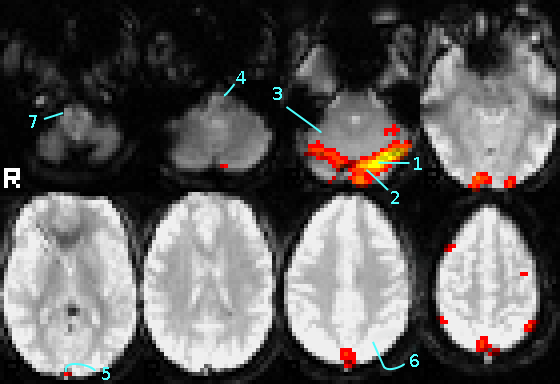
\includegraphics[scale=.85]{images/spm_hm}}
\subfigure[Sagittal Slice]{\label{fig:hm_canon_spm_x} 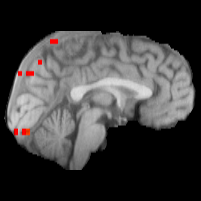
\includegraphics[scale=3]{images/spm_hm_x}}
\subfigure[Coronal Slice]{\label{fig:hm_canon_spm_y} 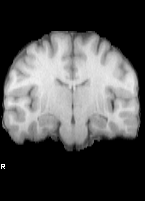
\includegraphics[scale=3]{images/spm_hm_y}}
\subfigure[Axial Slice]{\label{fig:hm_canon_spm_z} 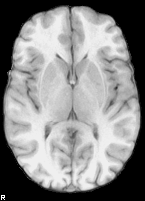
\includegraphics[scale=3]{images/spm_hm_z}}
\subfigure{\label{fig:scale_spm} 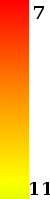
\includegraphics[scale=.5]{images/scale1}}
\caption[\acs{SPM} Results]{\acs{SPM} results. 
        Units of activation are in Student's $t$-scores; higher indicates higher
        assurance that the signal cannot have occurred through noise alone.}
\label{fig:hm_canon_spm}
\end{figure}

\begin{figure}[H]
\centering
\subfigure[Axial Slices]{\label{fig:hm_pfilter} 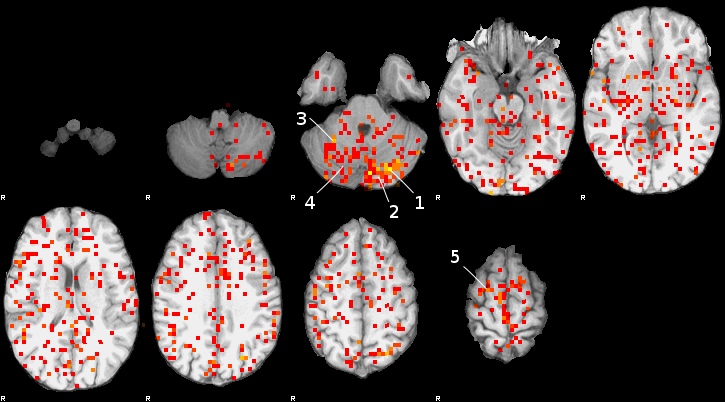
\includegraphics[scale=.85]{images/pfilter_hm}}
\subfigure[Sagittal Slice]{\label{fig:hm_canon_pfilter_x} 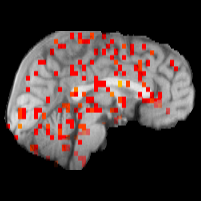
\includegraphics[scale=3]{images/pfilter_hm_x}}
\subfigure[Coronal Slice]{\label{fig:hm_canon_pfilter_y} 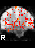
\includegraphics[scale=3]{images/pfilter_hm_y}}
\subfigure[Axial Slice]{\label{fig:hm_canon_pfilter_z} 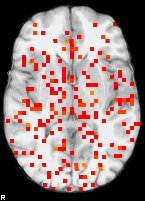
\includegraphics[scale=3]{images/pfilter_hm_z}}
\subfigure{\label{fig:scale_pfilter} 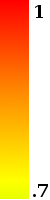
\includegraphics[scale=.5]{images/scale2}}
\caption[Particle Filter results measured in normalized error.]
    {Particle Filter results measured in normalized error.
        Units of match is normalized residual where the lowest (best) levels shown are
        $0.7$ and the highest error shown (threshold) is $1$.
        Sagittal, coronal and axial slices are shwon in \autoref{fig:hm_canon_pfilter_x}.}
\label{fig:hm_canon_pfilter}
\end{figure}

%\begin{figure}[H]
%\centering
%\subfigure[]{\label{fig:hm_pfilter85} 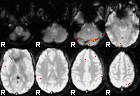
\includegraphics[scale=.75]{images/pfilter85_hm}}
%\subfigure[]{\label{fig:hm_canon_pfilter85_x} 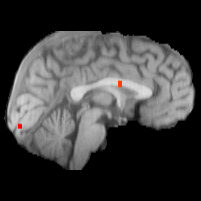
\includegraphics[scale=3]{images/pfilter_hm85_x}}
%\subfigure[]{\label{fig:hm_canon_pfilter85_y} 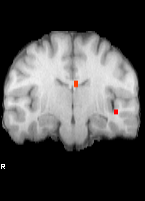
\includegraphics[scale=3]{images/pfilter_hm85_y}}
%\subfigure[]{\label{fig:hm_canon_pfilter85_z} 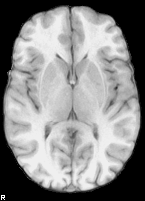
\includegraphics[scale=3]{images/pfilter_hm85_z}}
%\subfigure{\label{fig:scale_pfilter85} 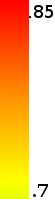
\includegraphics[scale=.5]{images/scale3}}
%\caption{Sagittal, coronal and axial (\autoref{fig:hm_canon_pfilter_x} \autoref{fig:hm_canon_pfilter_y}
%         \autoref{fig:hm_canon_pfilter_x}), as well as a series of axial slices, \autoref{fig:hm_pfilter}.
%         Units of match is normalized residual. The lowest (best) levels were $.7$.
%         The highest error shown is $.85$.}
%\label{fig:hm_canon_pfilter85}
%\end{figure}

\begin{figure}[H]
\centering
\subfigure[Axial Slices]{\label{fig:hm_mi} 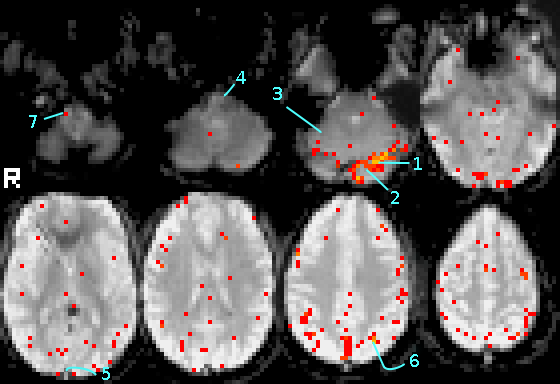
\includegraphics[scale=.85]{images/mi_hm}}
\subfigure[Sagittal Slice]{\label{fig:hm_canon_mi_x} 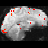
\includegraphics[scale=3]{images/mi_hm_x}}
\subfigure[Coronal Slice]{\label{fig:hm_canon_mi_y} 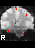
\includegraphics[scale=3]{images/mi_hm_y}}
\subfigure[Axial Slice]{\label{fig:hm_canon_mi_z} 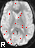
\includegraphics[scale=3]{images/mi_hm_z}}
\subfigure{\label{fig:scale_mi} 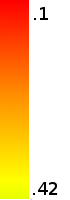
\includegraphics[scale=.5]{images/scale4}}
\caption[Particle Filter results measured in \ac{MI}.]
        {Particle Filter results measured in \ac{MI}.
         Units of match is bits (standard for base-2 \ac{MI}). The highest (best) levels are
         $0.42$ and the worst shown (threshold) is $0.1$.}
\label{fig:hm_canon_pfilter_mi}
\end{figure}

%37-14-7
\begin{figure}
\centering
\subfigure[Particle Filter]{\label{fig:comp1pfilter} 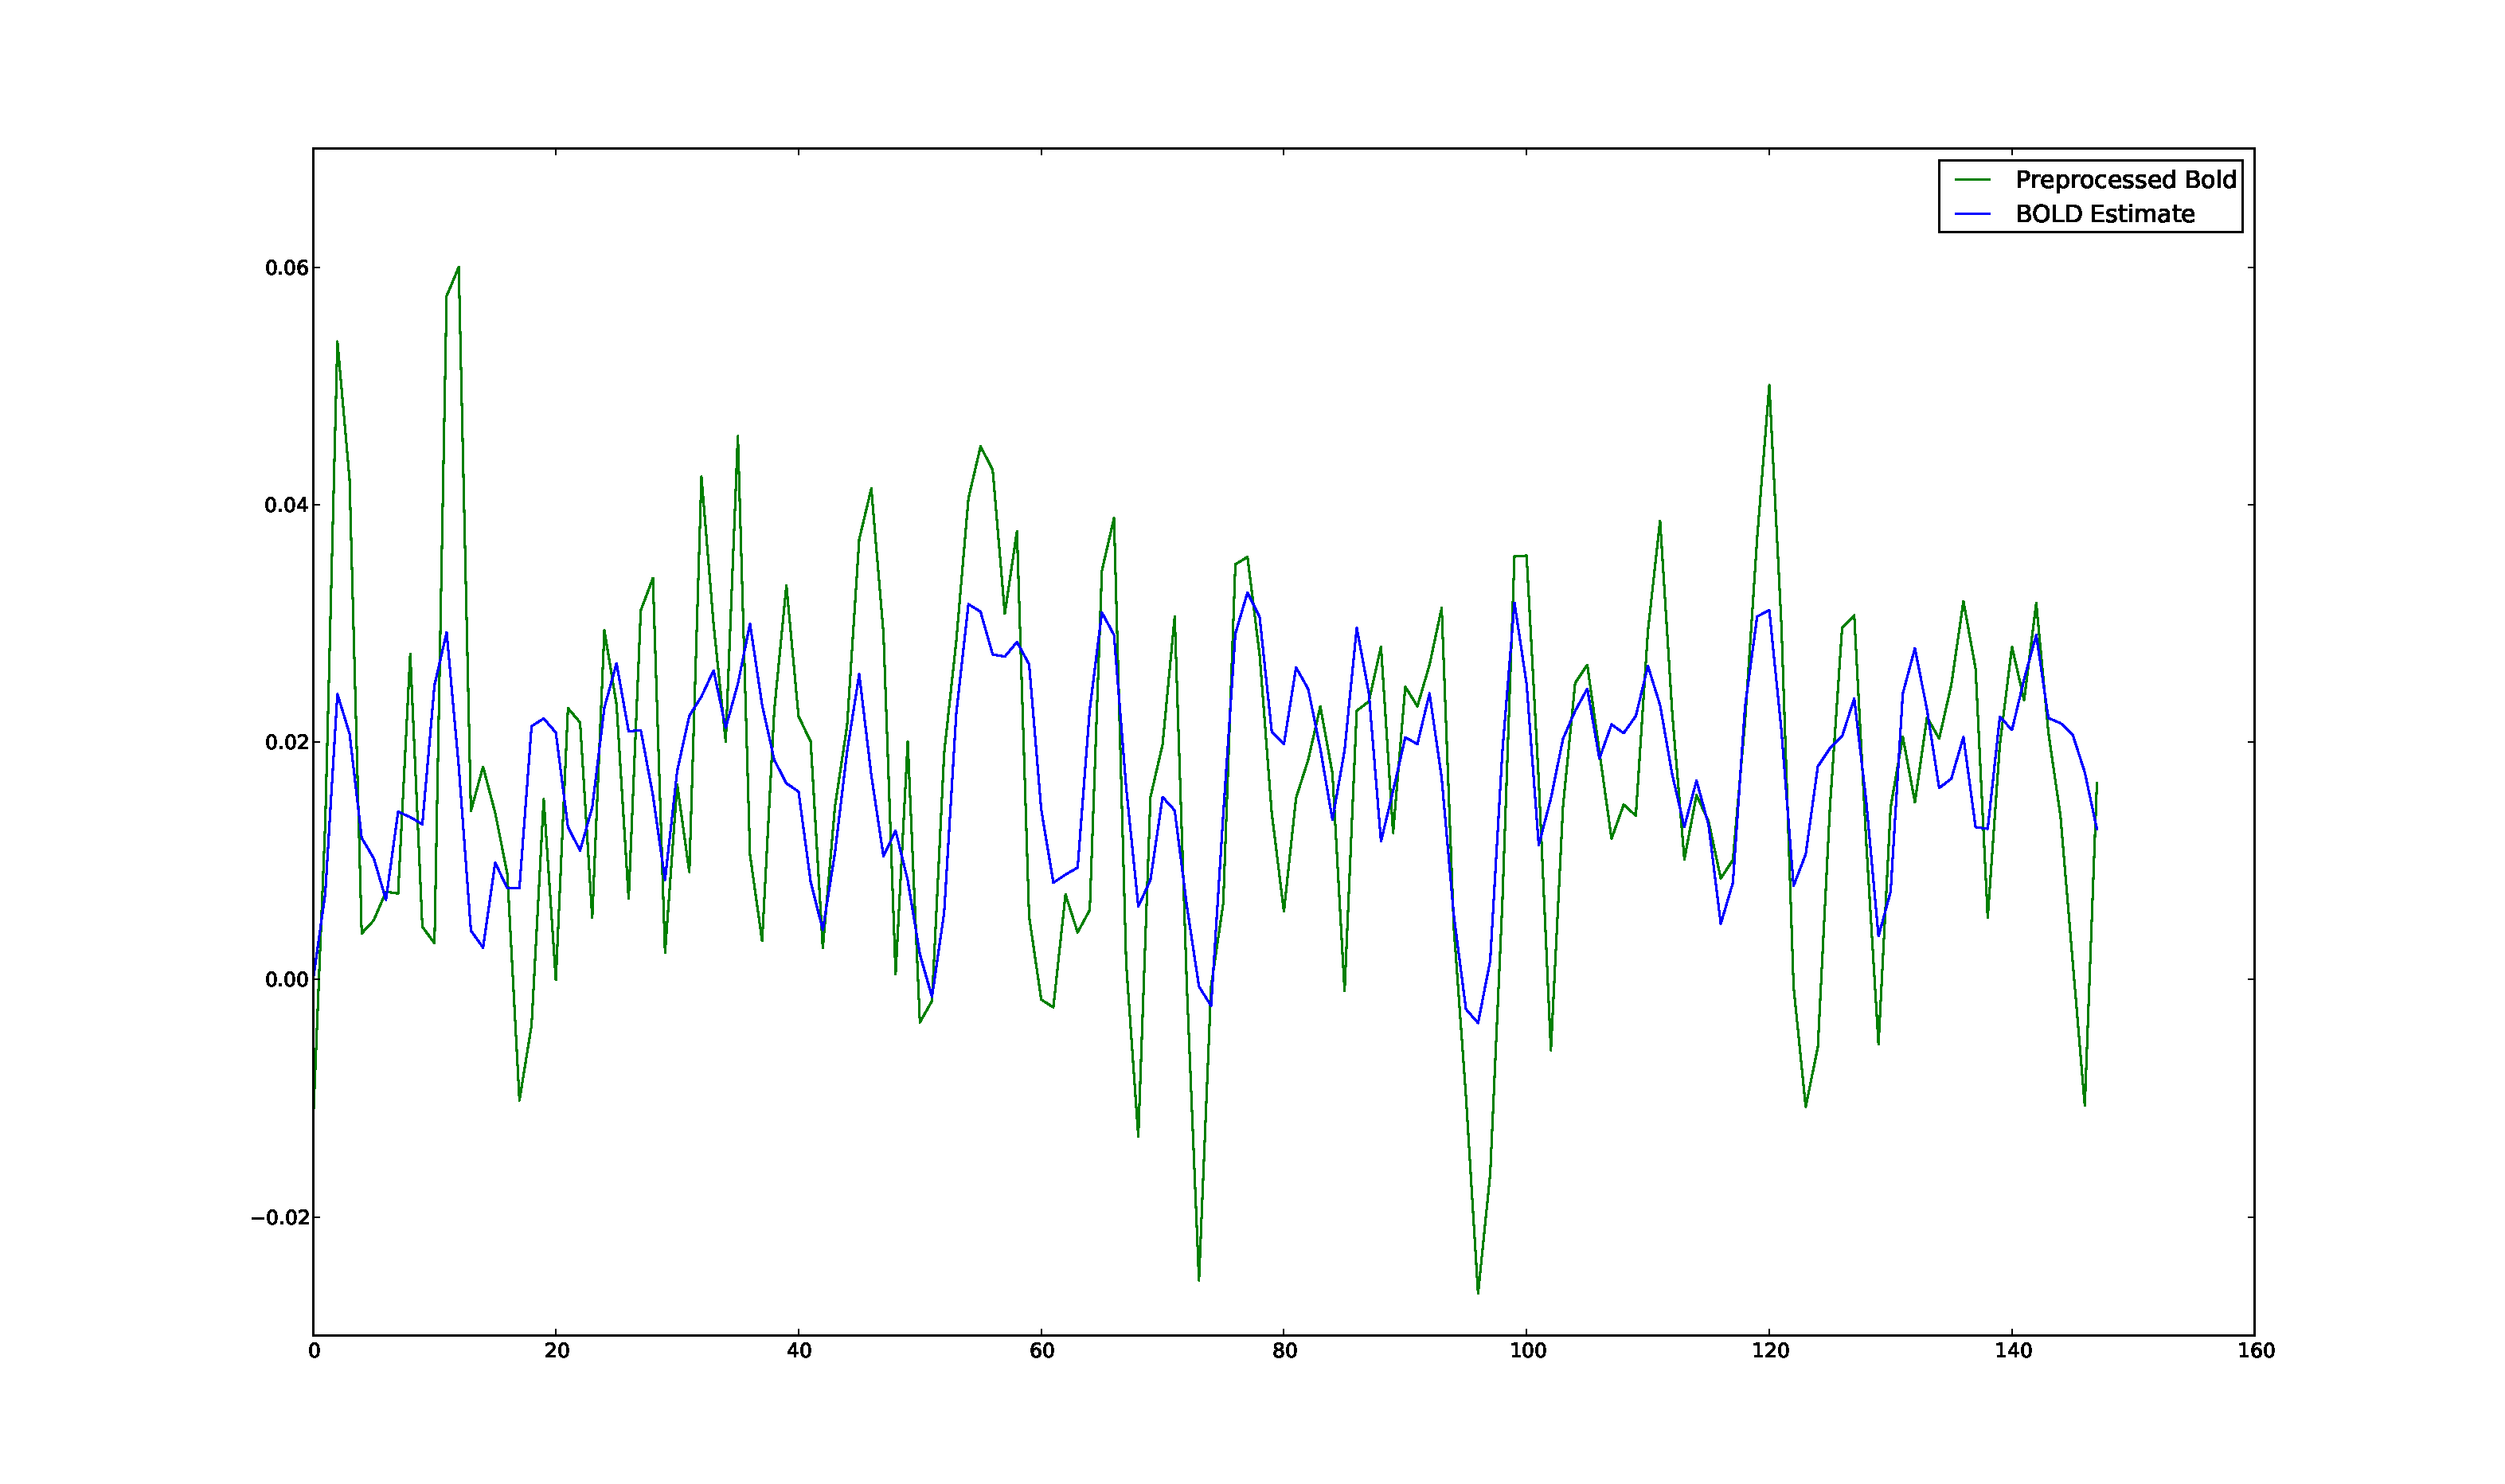
\includegraphics[clip=true,trim=5cm 2.5cm 4cm 3cm,width=.93\textwidth]{images/1_pfilter_37_14_7}}
\subfigure[SPM]{\label{fig:comp1spm} 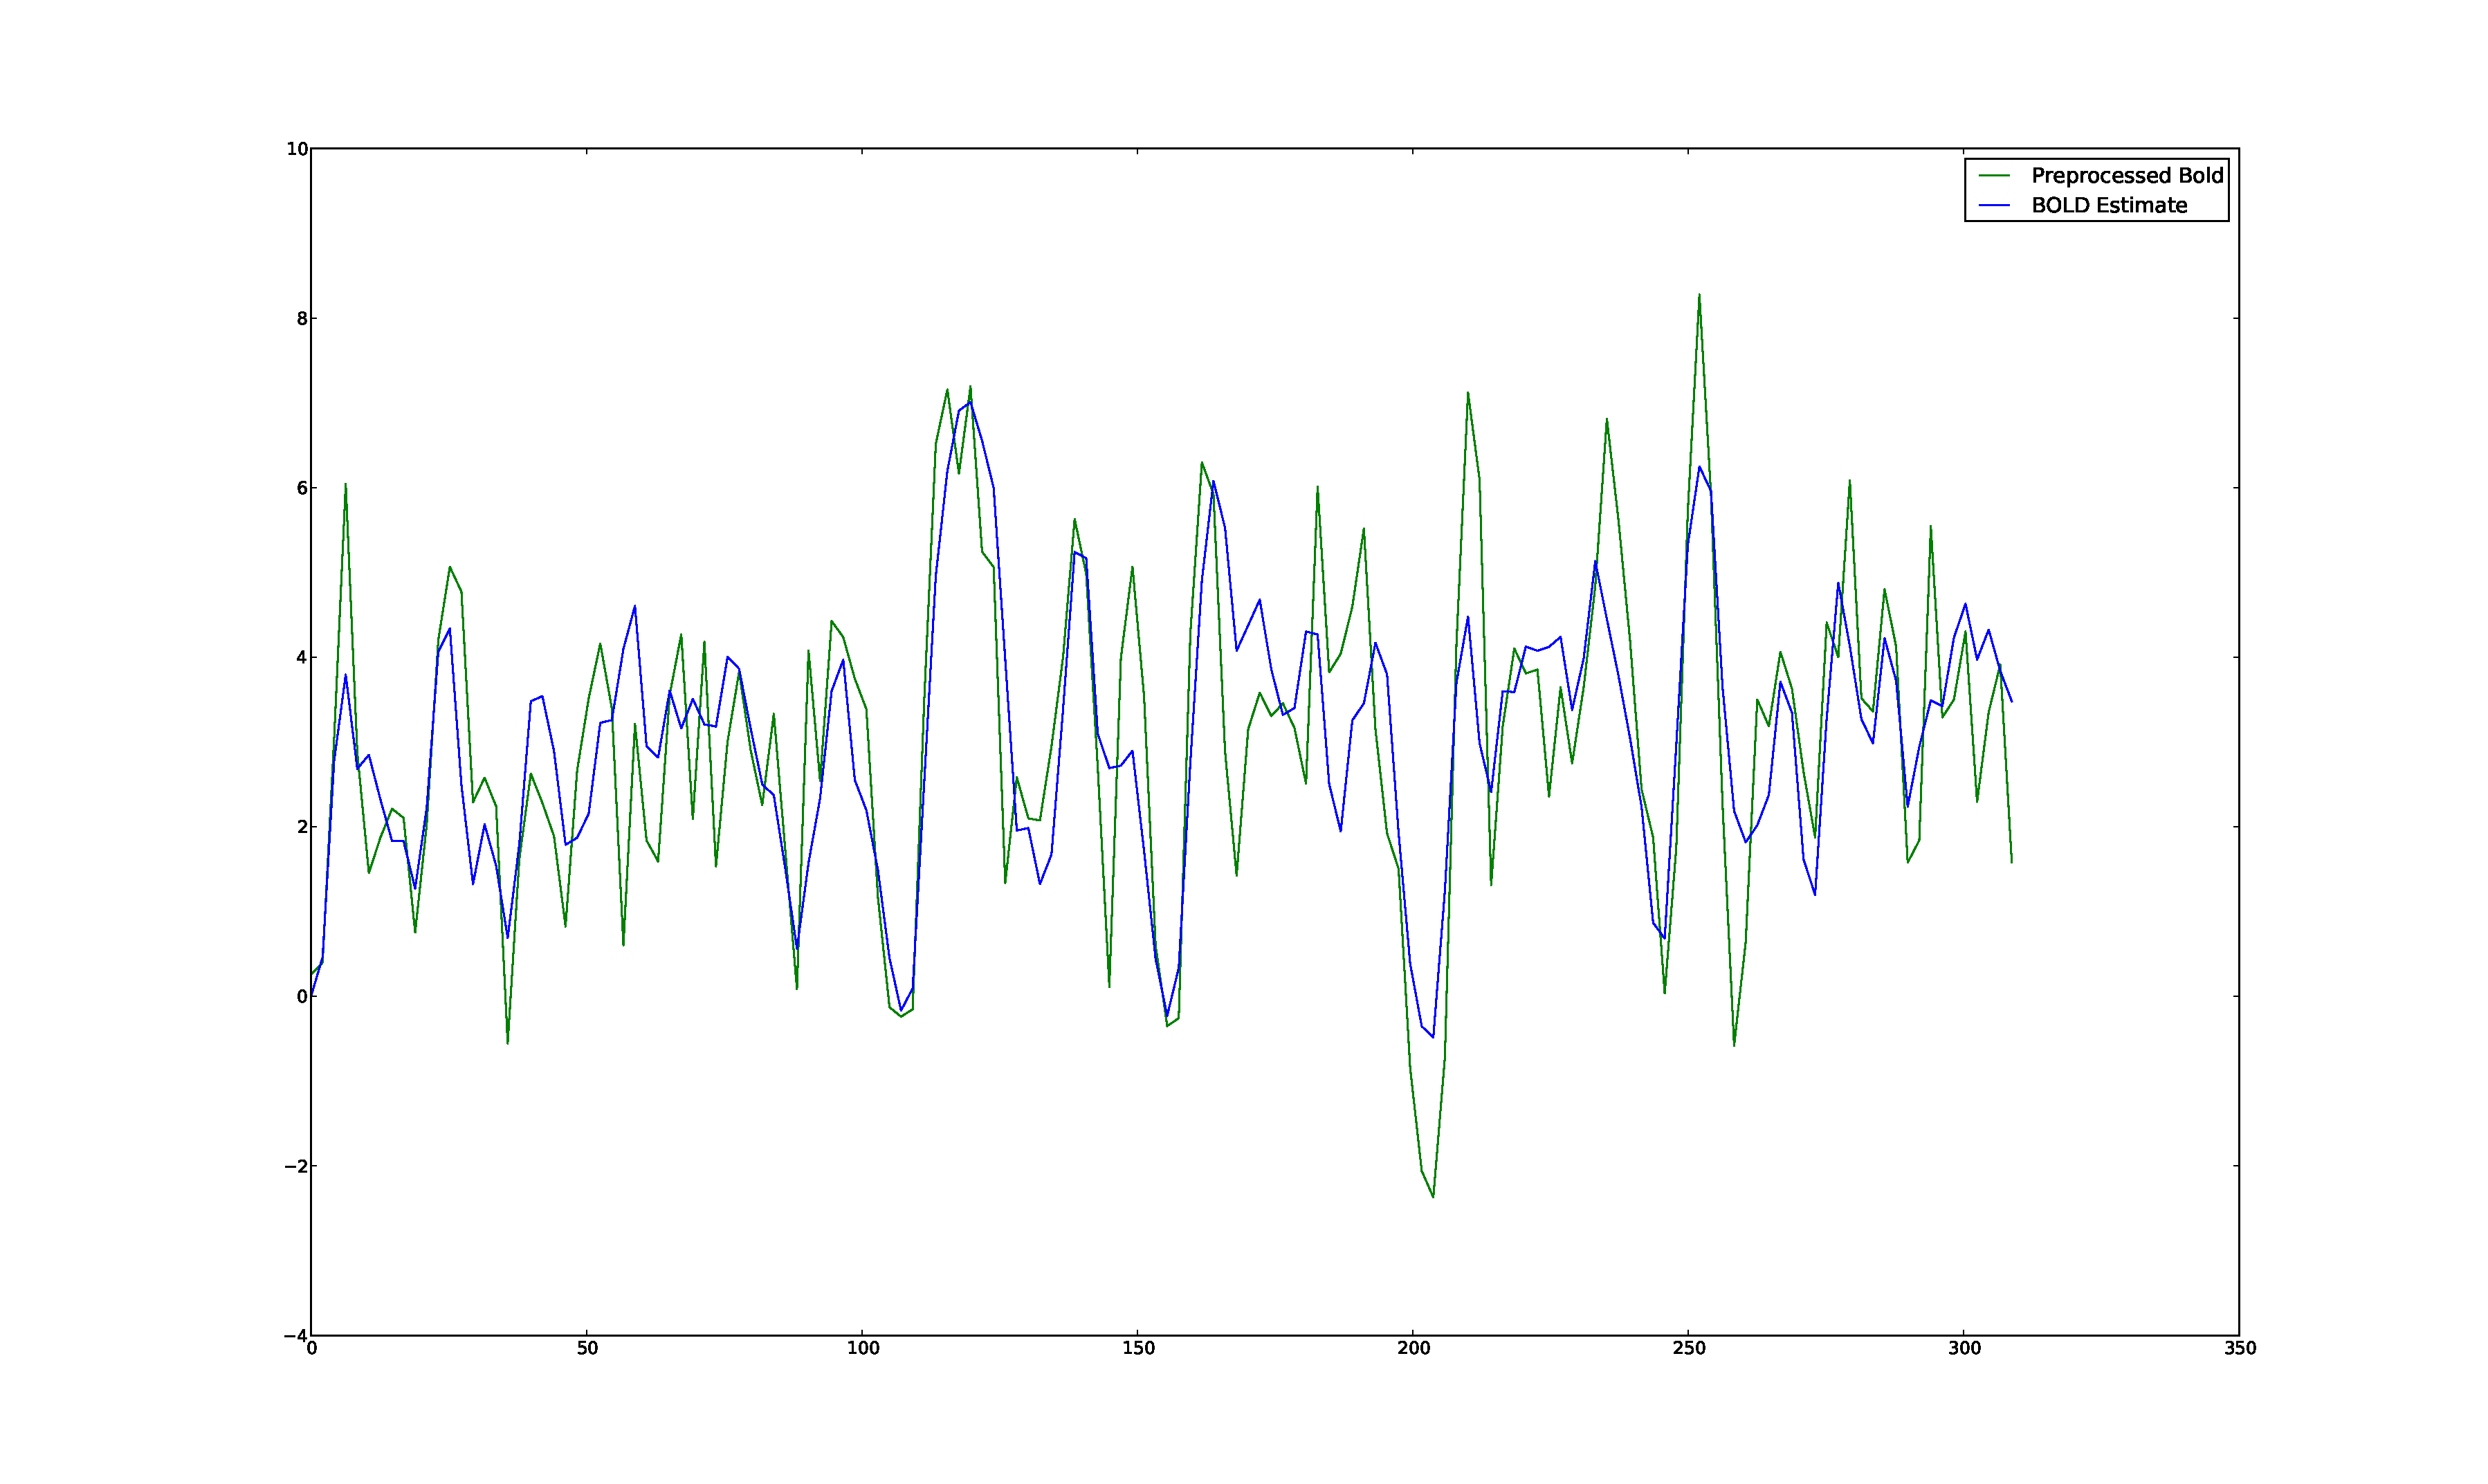
\includegraphics[clip=true,trim=5cm 2.5cm 4cm 3cm,width=.93\textwidth]{images/1_spm_37_14_7}}
\caption[Time Series Comparison, Section 1]{Time Series Comparison, Section 1.
Estimated vs. Actual \ac{BOLD} response. $t$-Score: $10.71$, \ac{MI}: $0.33$, Residual: $0.72$.}
\label{fig:comp1}
\end{figure}

%34-12-7
\begin{figure}
\centering
\subfigure[Particle Filter]{\label{fig:comp2pfilter} 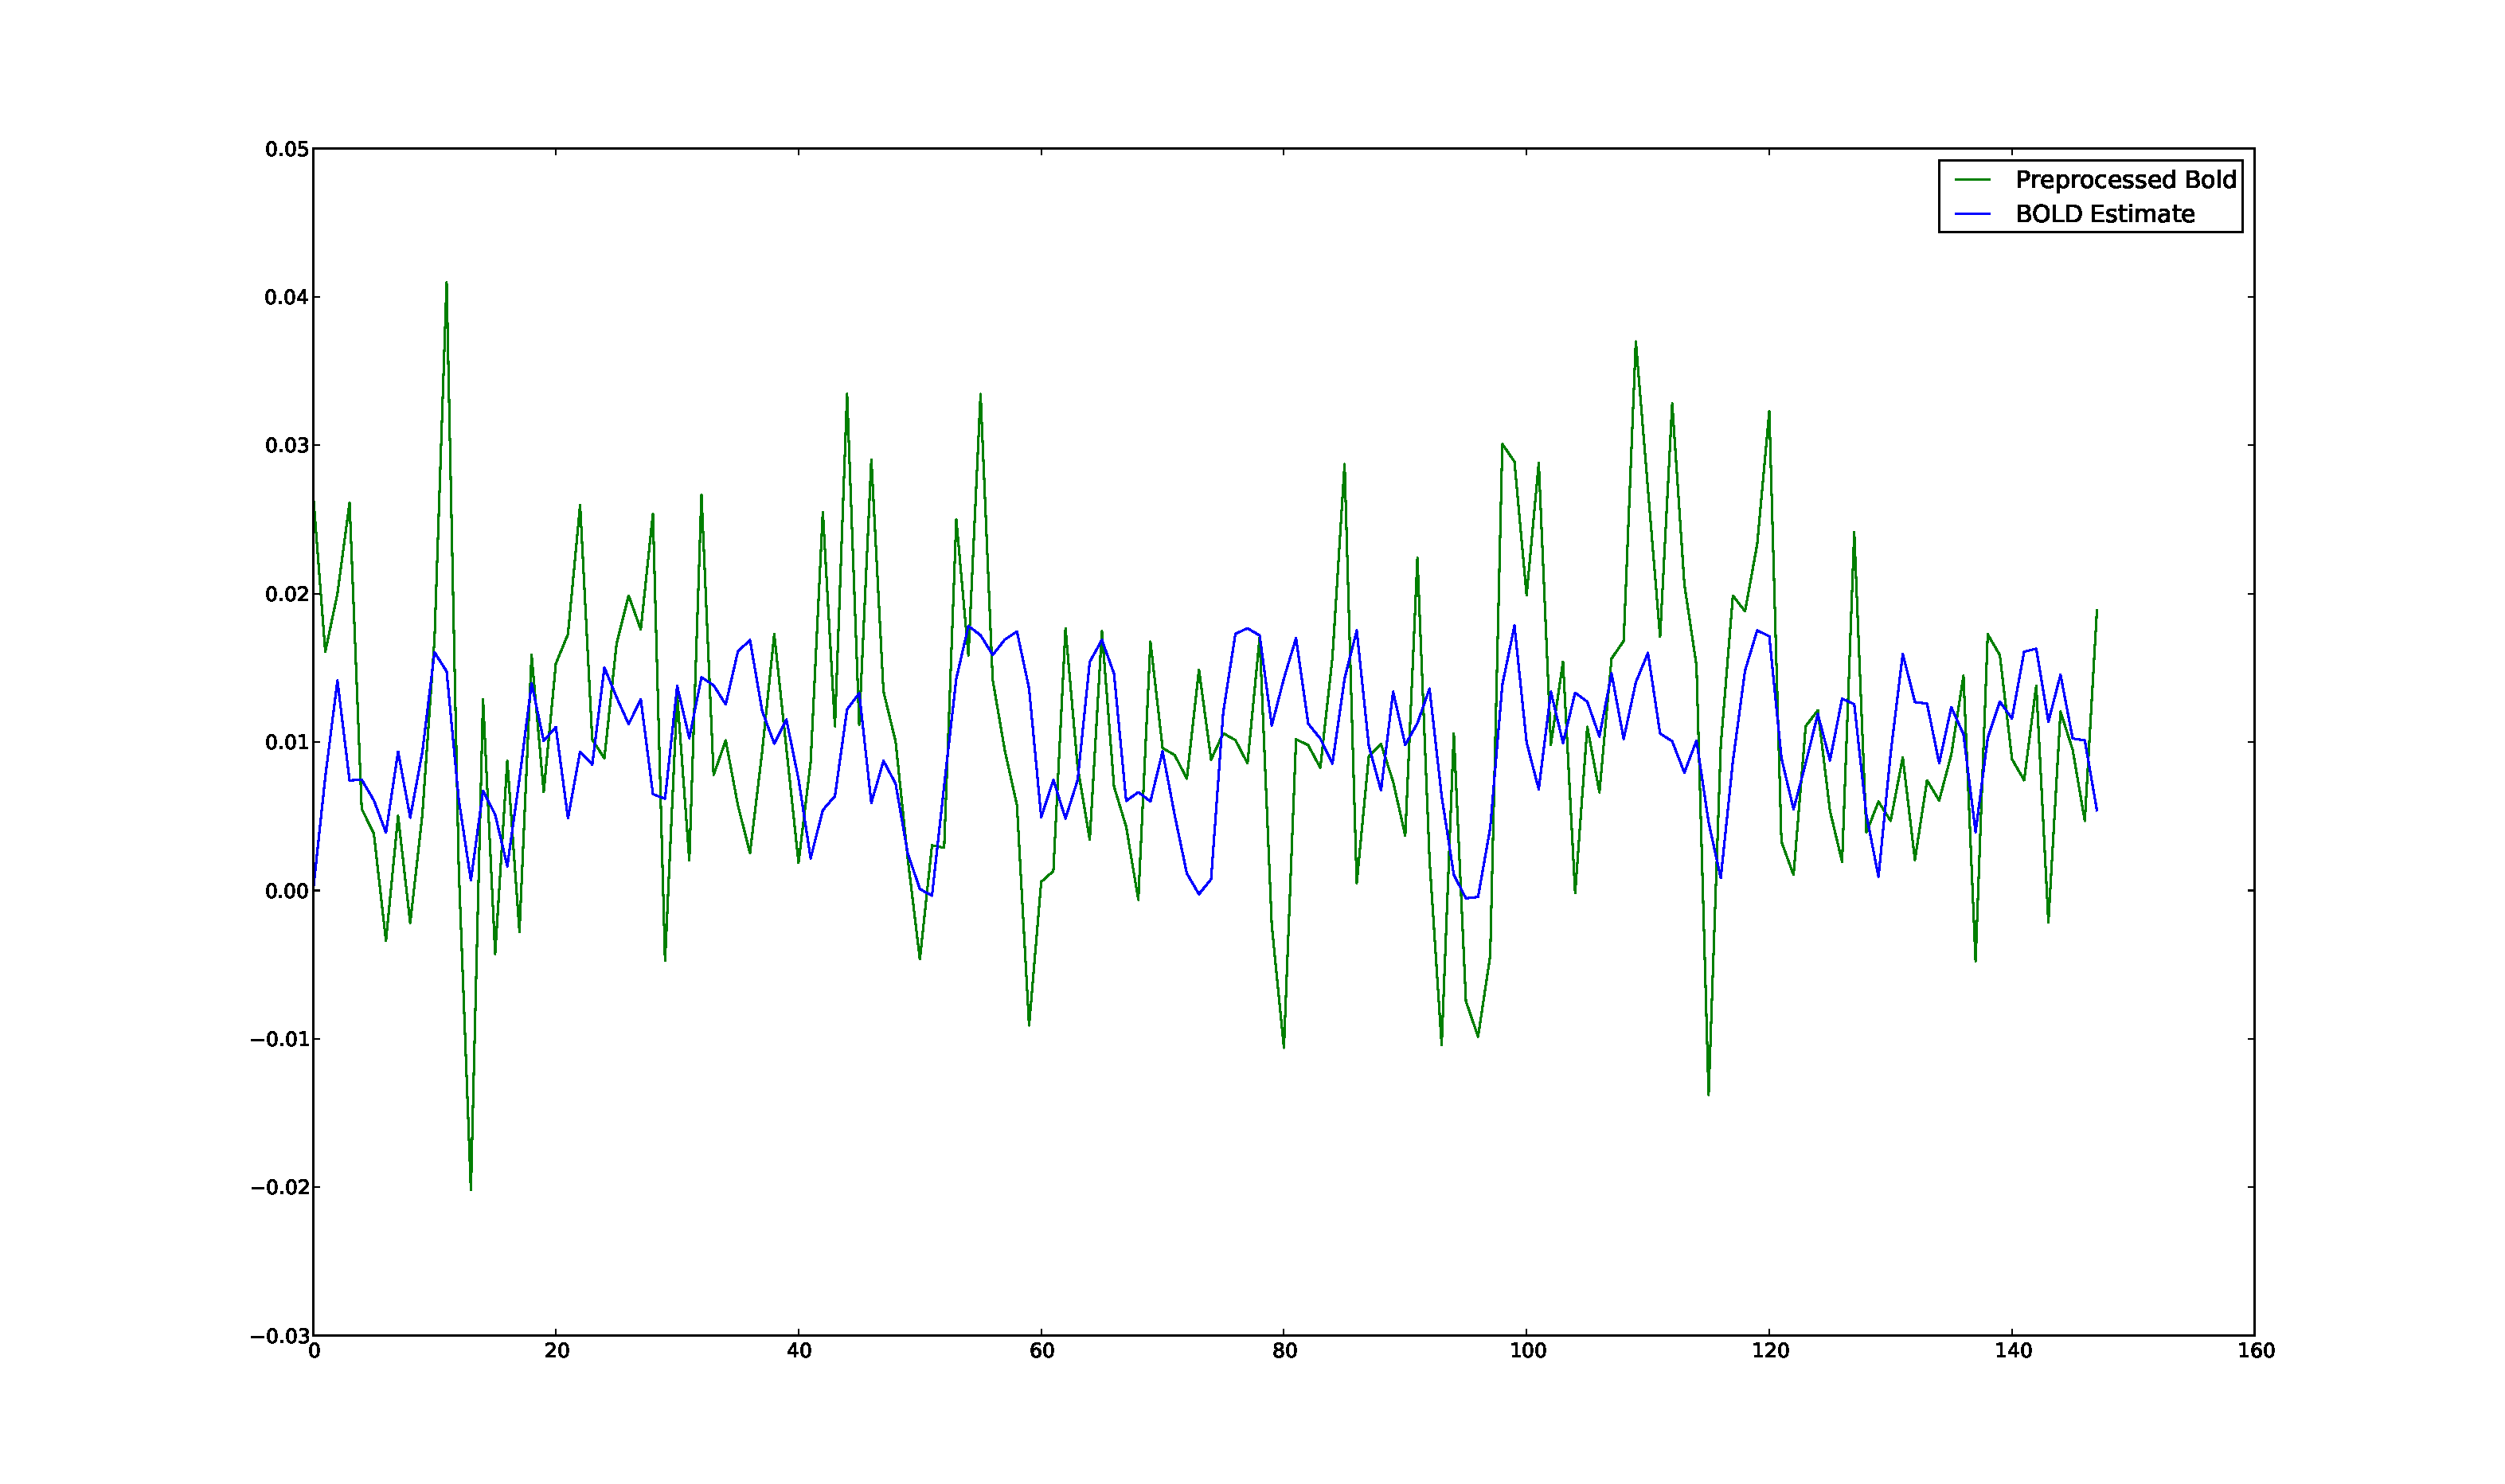
\includegraphics[clip=true,trim=5cm 2.5cm 4cm 3cm,width=.93\textwidth]{images/2_pfilter_34_12_7}}
\subfigure[SPM]{\label{fig:comp2spm} 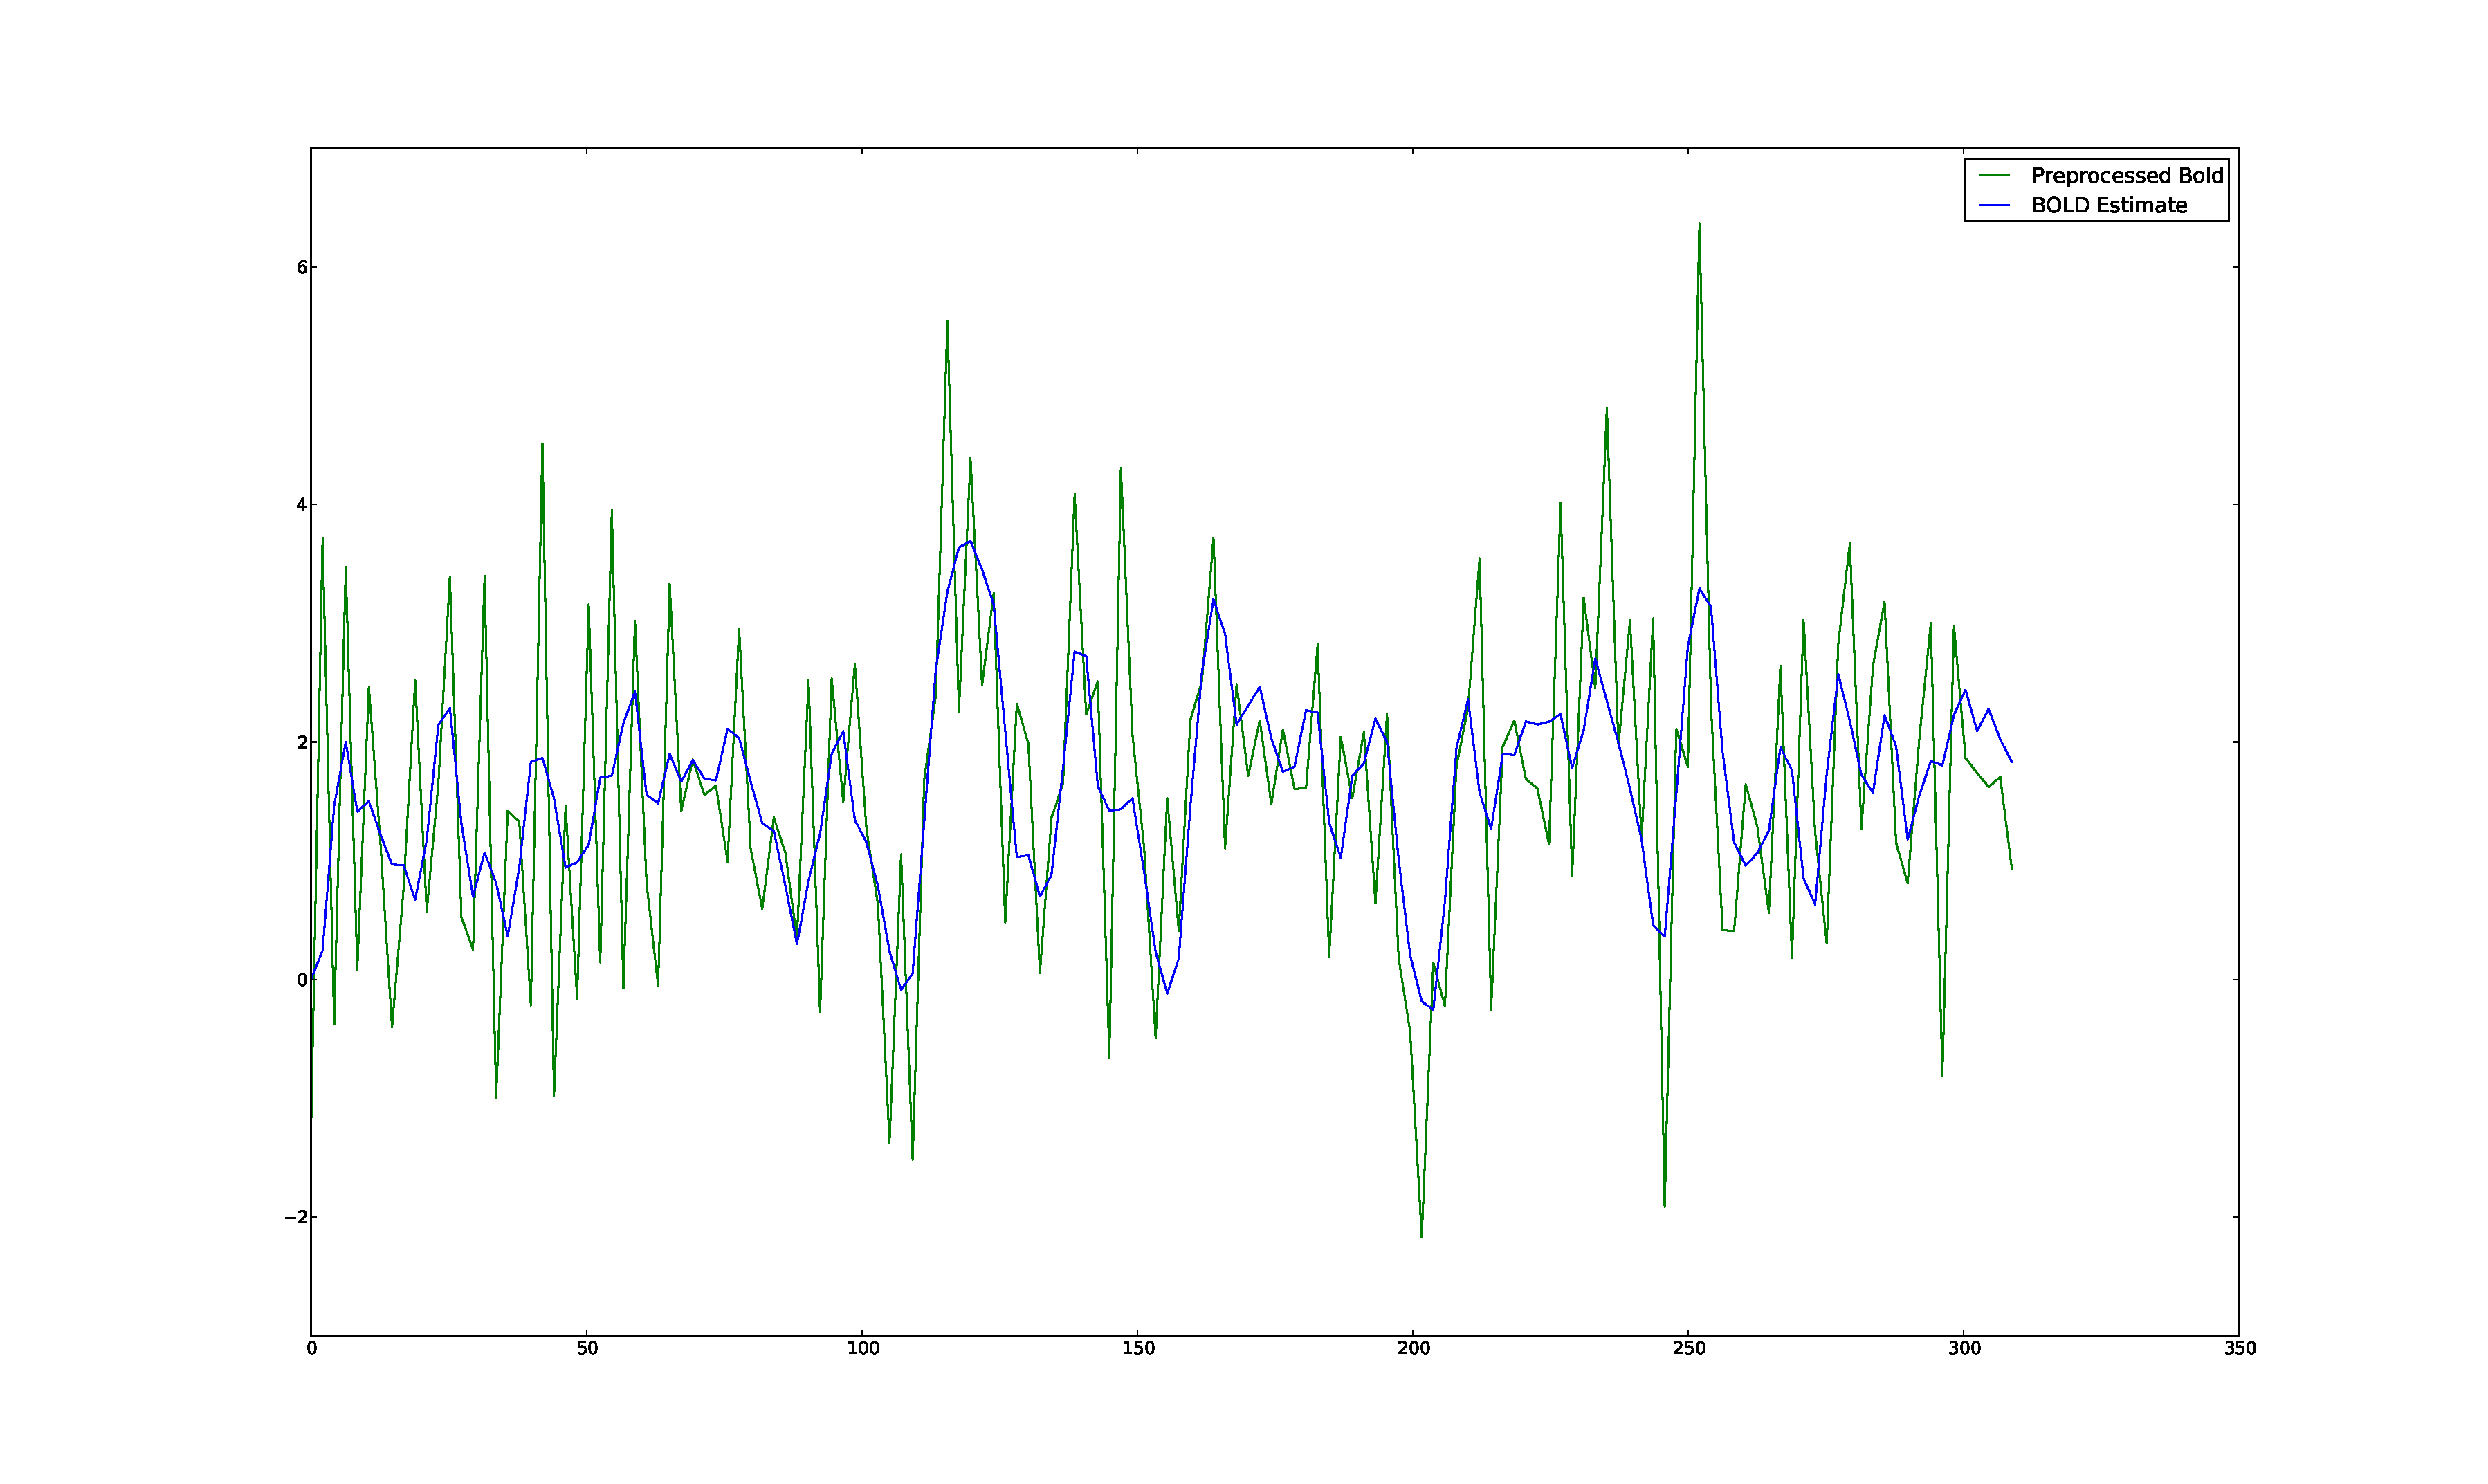
\includegraphics[clip=true,trim=5cm 2.5cm 4cm 3cm,width=.93\textwidth]{images/2_spm_34_12_7}}
\caption[Time Series Comparison, Section 2]{Time Series Comparison, Section 2.
Estimated vs. Actual \ac{BOLD} response. $t$-Score: $6.97$, \ac{MI}: $0.04$, Residual: $1.02$.}
\label{fig:comp2}
\end{figure}

%23-21-7
\begin{figure}
\centering
\subfigure[Particle Filter]{\label{fig:comp3pfilter} 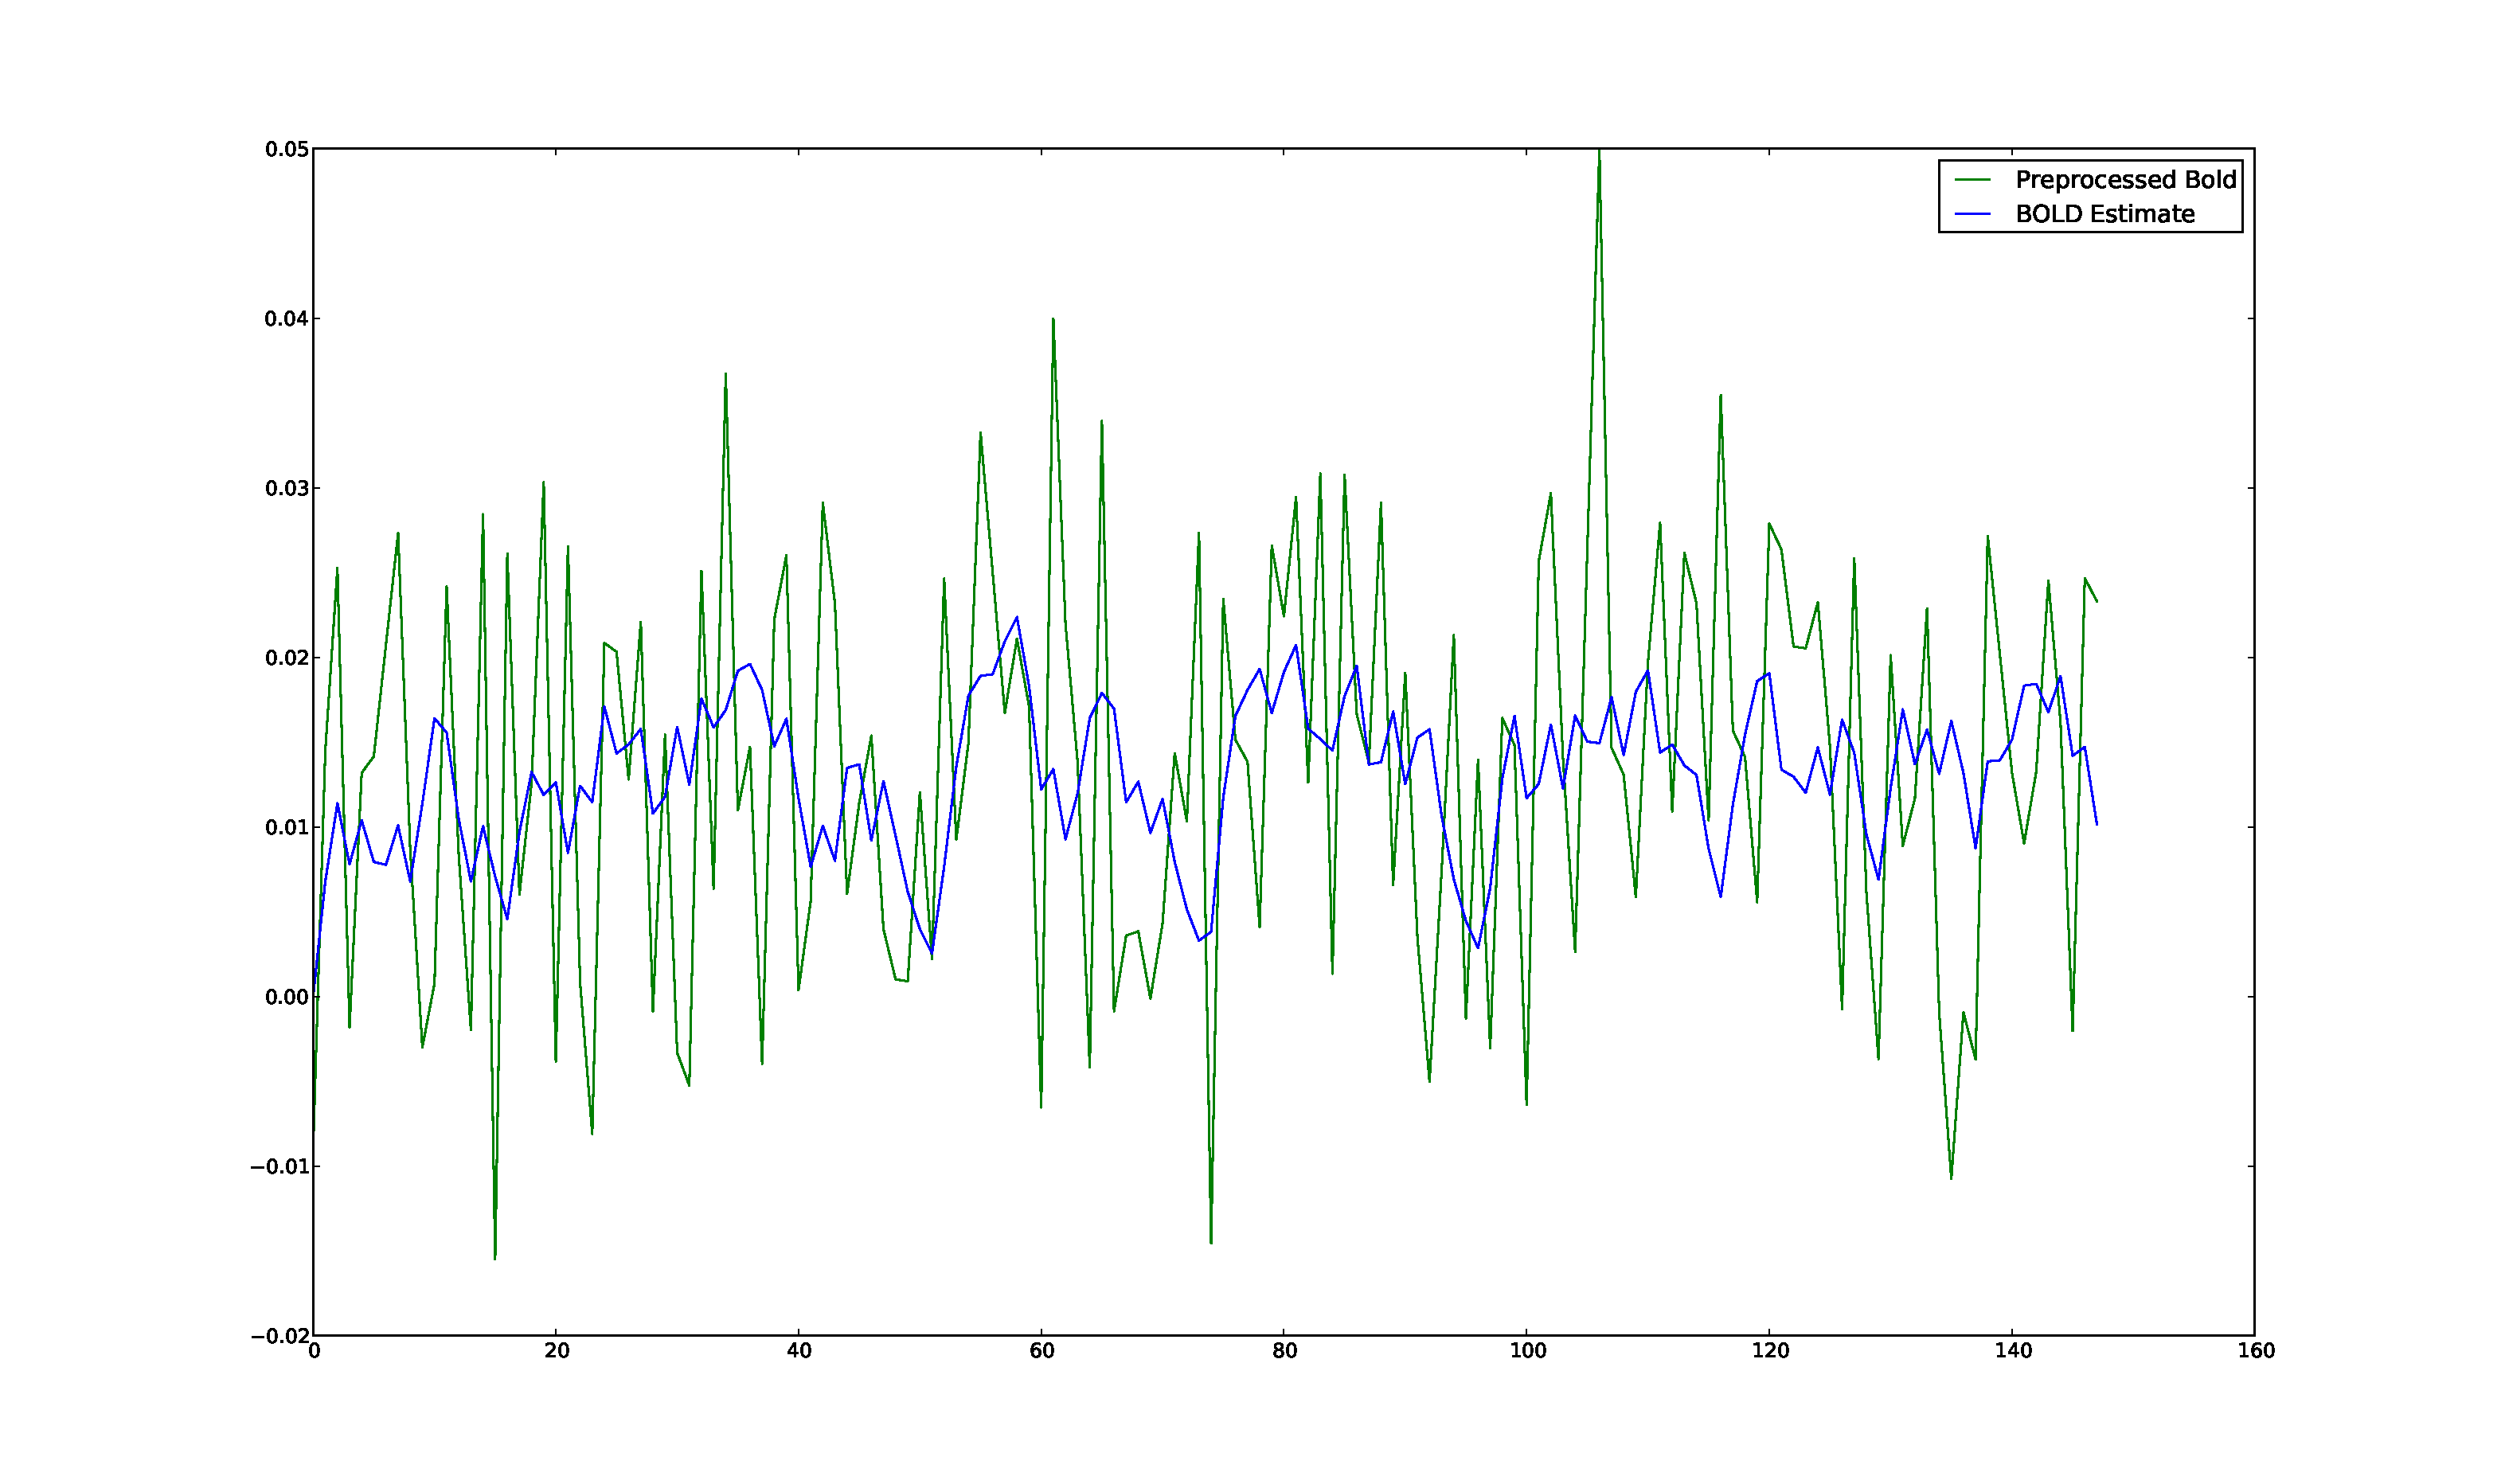
\includegraphics[clip=true,trim=5cm 2.5cm 4cm 3cm,width=.93\textwidth]{images/3_pfilter_23_21_7}}
\subfigure[SPM]{\label{fig:comp3spm} 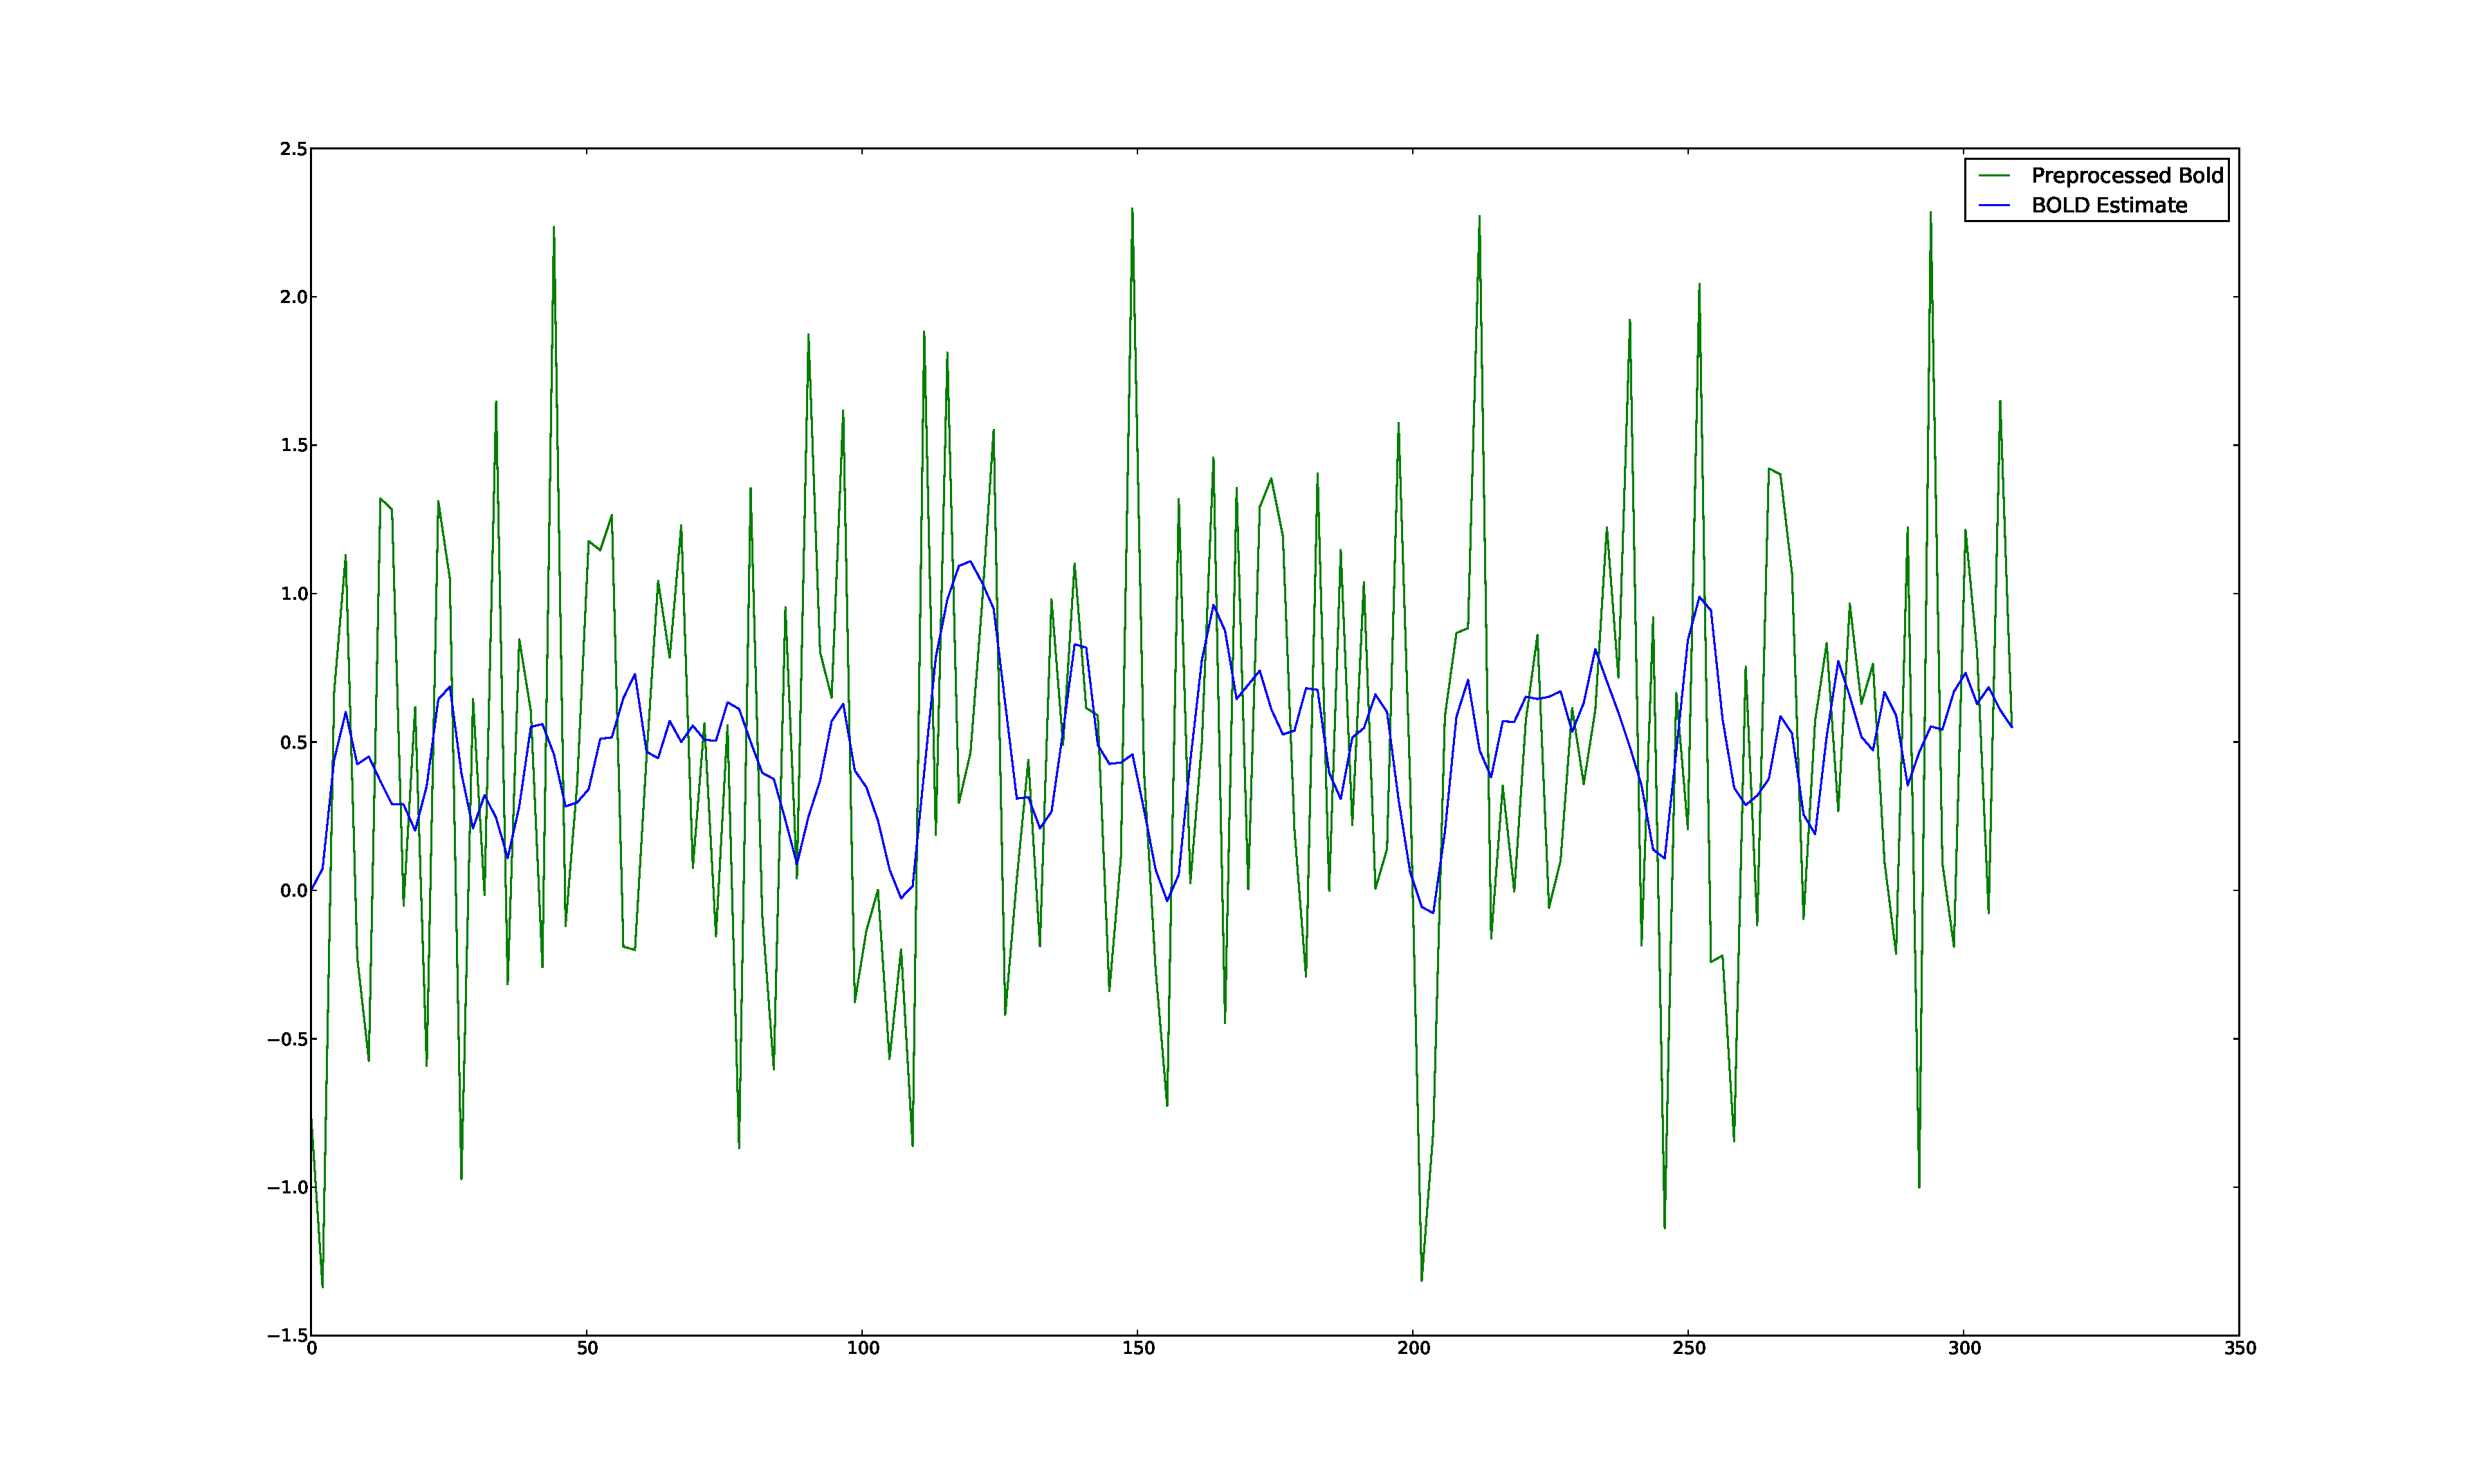
\includegraphics[clip=true,trim=5cm 2.5cm 4cm 3cm,width=.93\textwidth]{images/3_spm_23_21_7}}
\caption[Time Series Comparison, Section 3]{Time Series Comparison, Section 3.
Estimated vs. Actual \ac{BOLD} response. $t$-Score: $2.85$, \ac{MI}: $-0.03$, Residual: $0.81$.}
\label{fig:comp3}
\end{figure}

%33-30-4
\begin{figure}[H]
\centering
\subfigure[Particle Filter]{\label{fig:comp4pfilter} 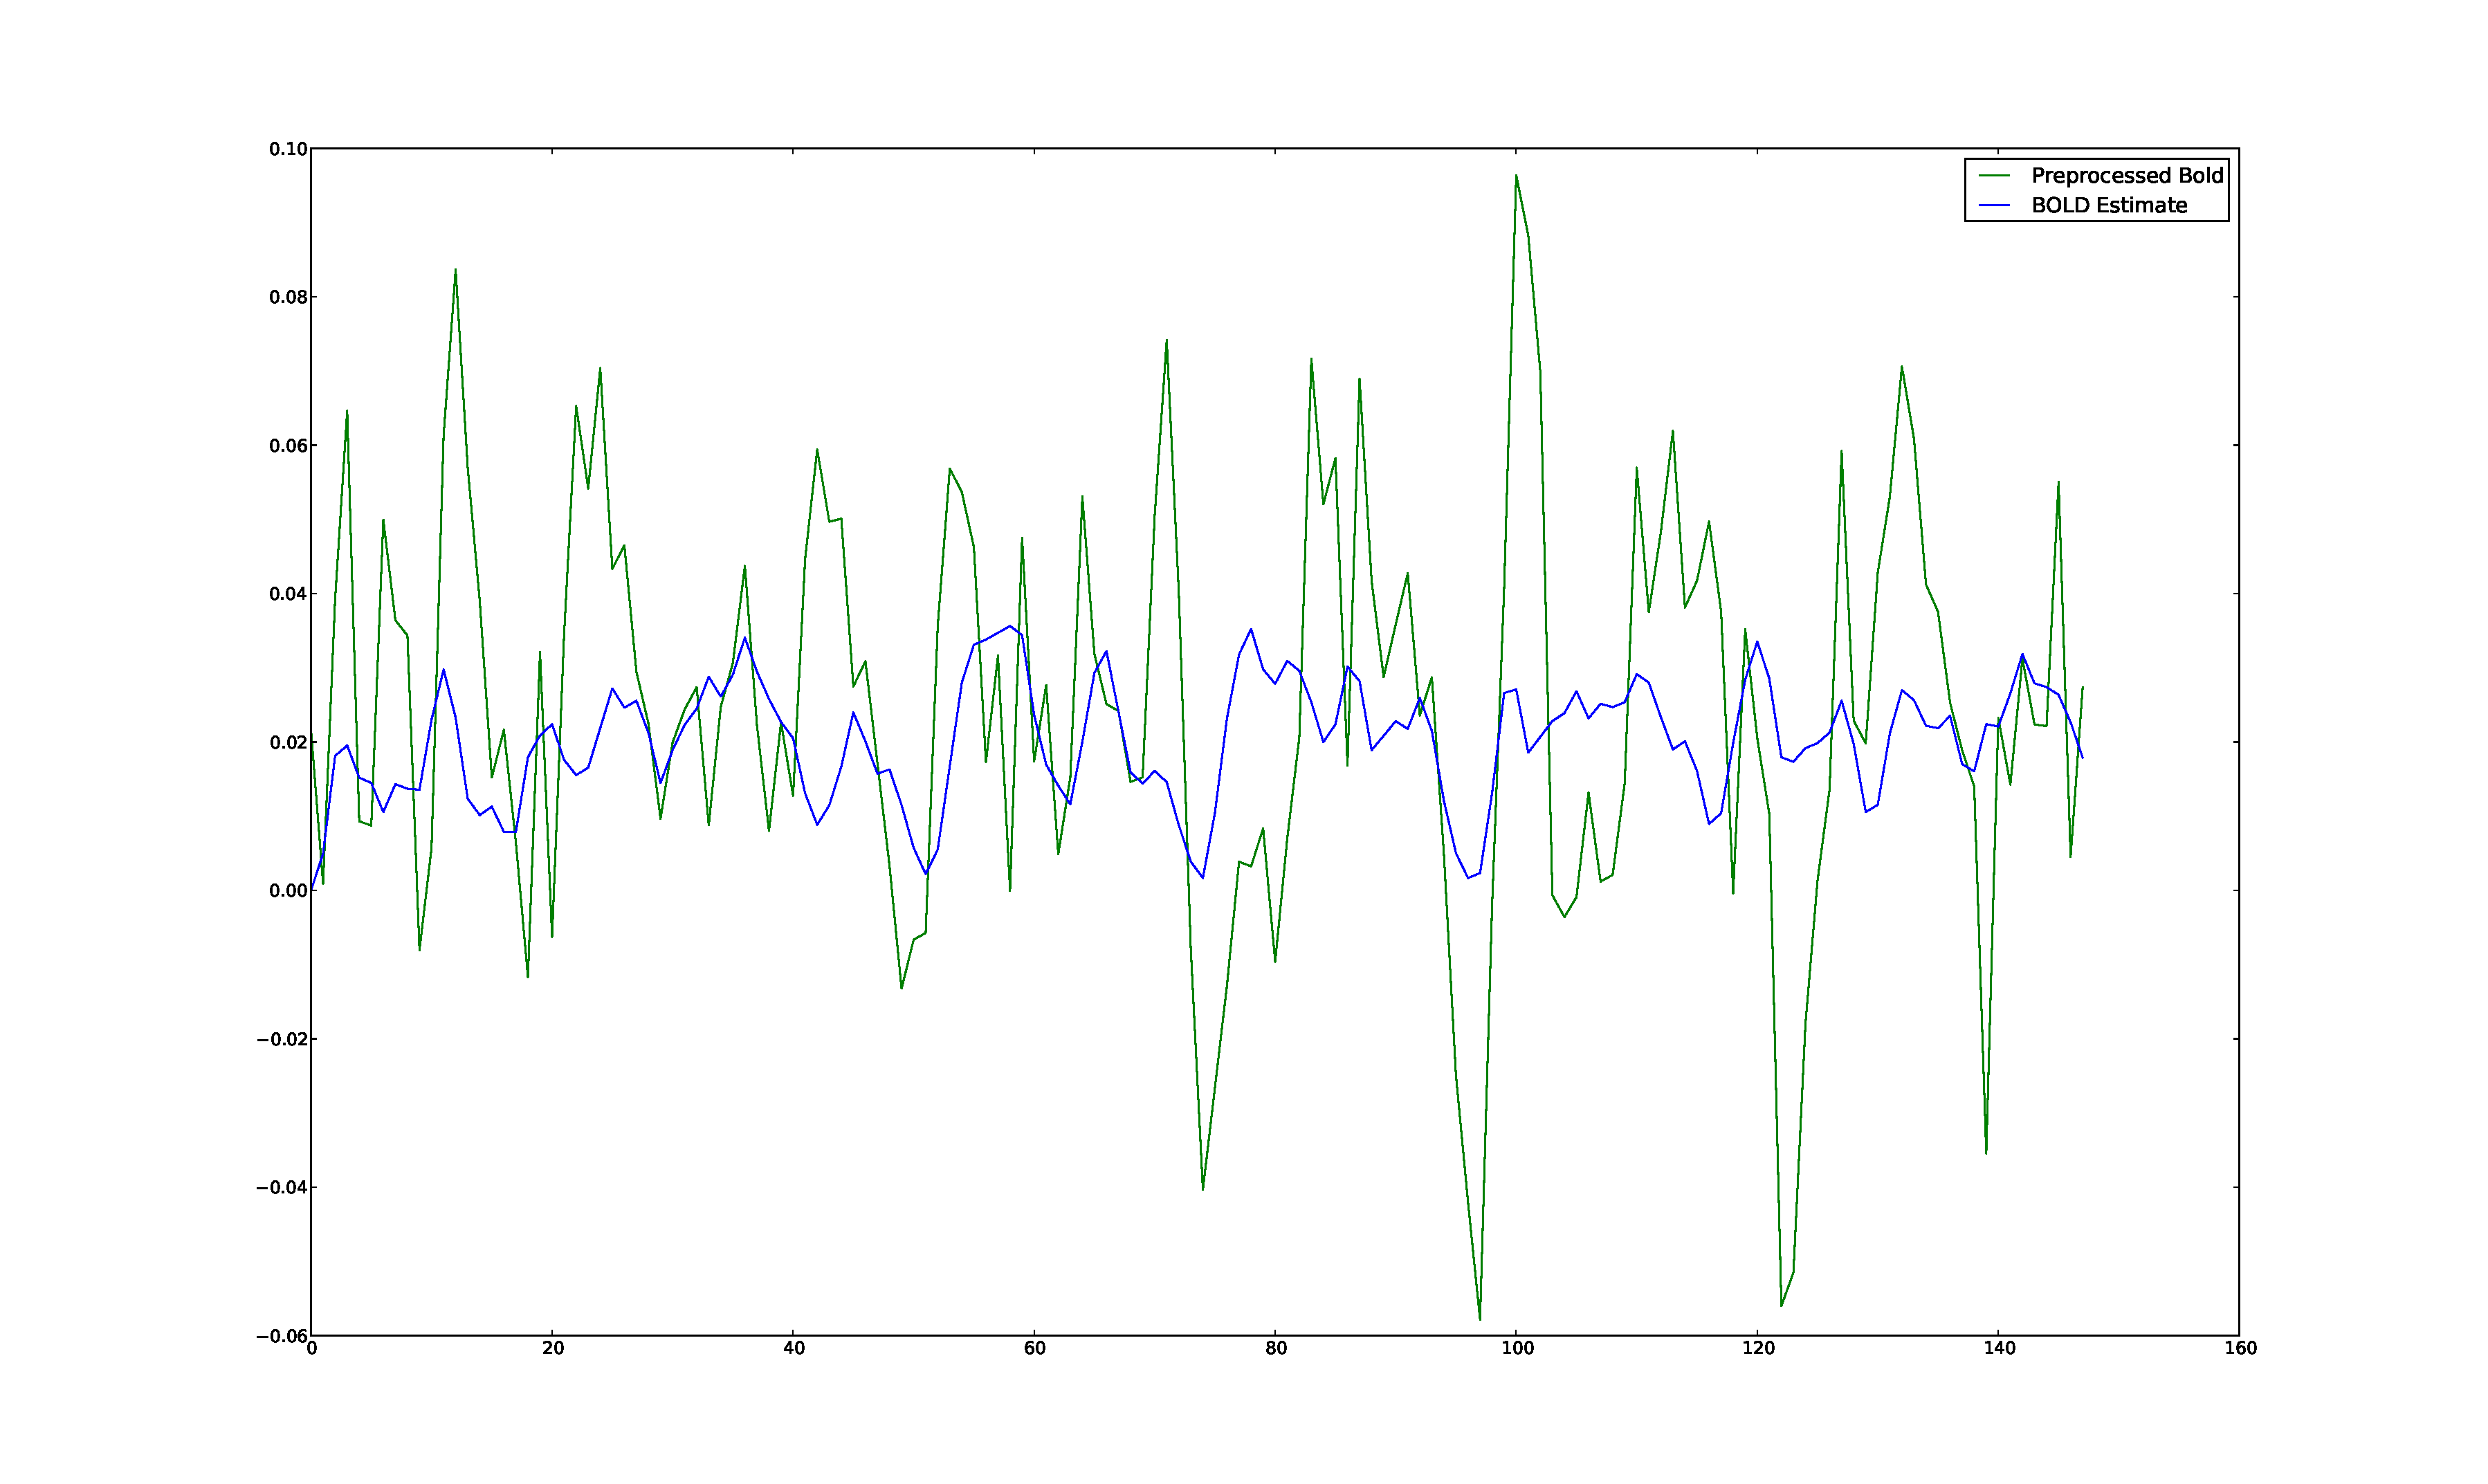
\includegraphics[clip=true,trim=5cm 2.5cm 4cm 3cm,width=.93\textwidth]{images/4_pfilter_26_15_7}}
\subfigure[SPM]{\label{fig:comp4spm} 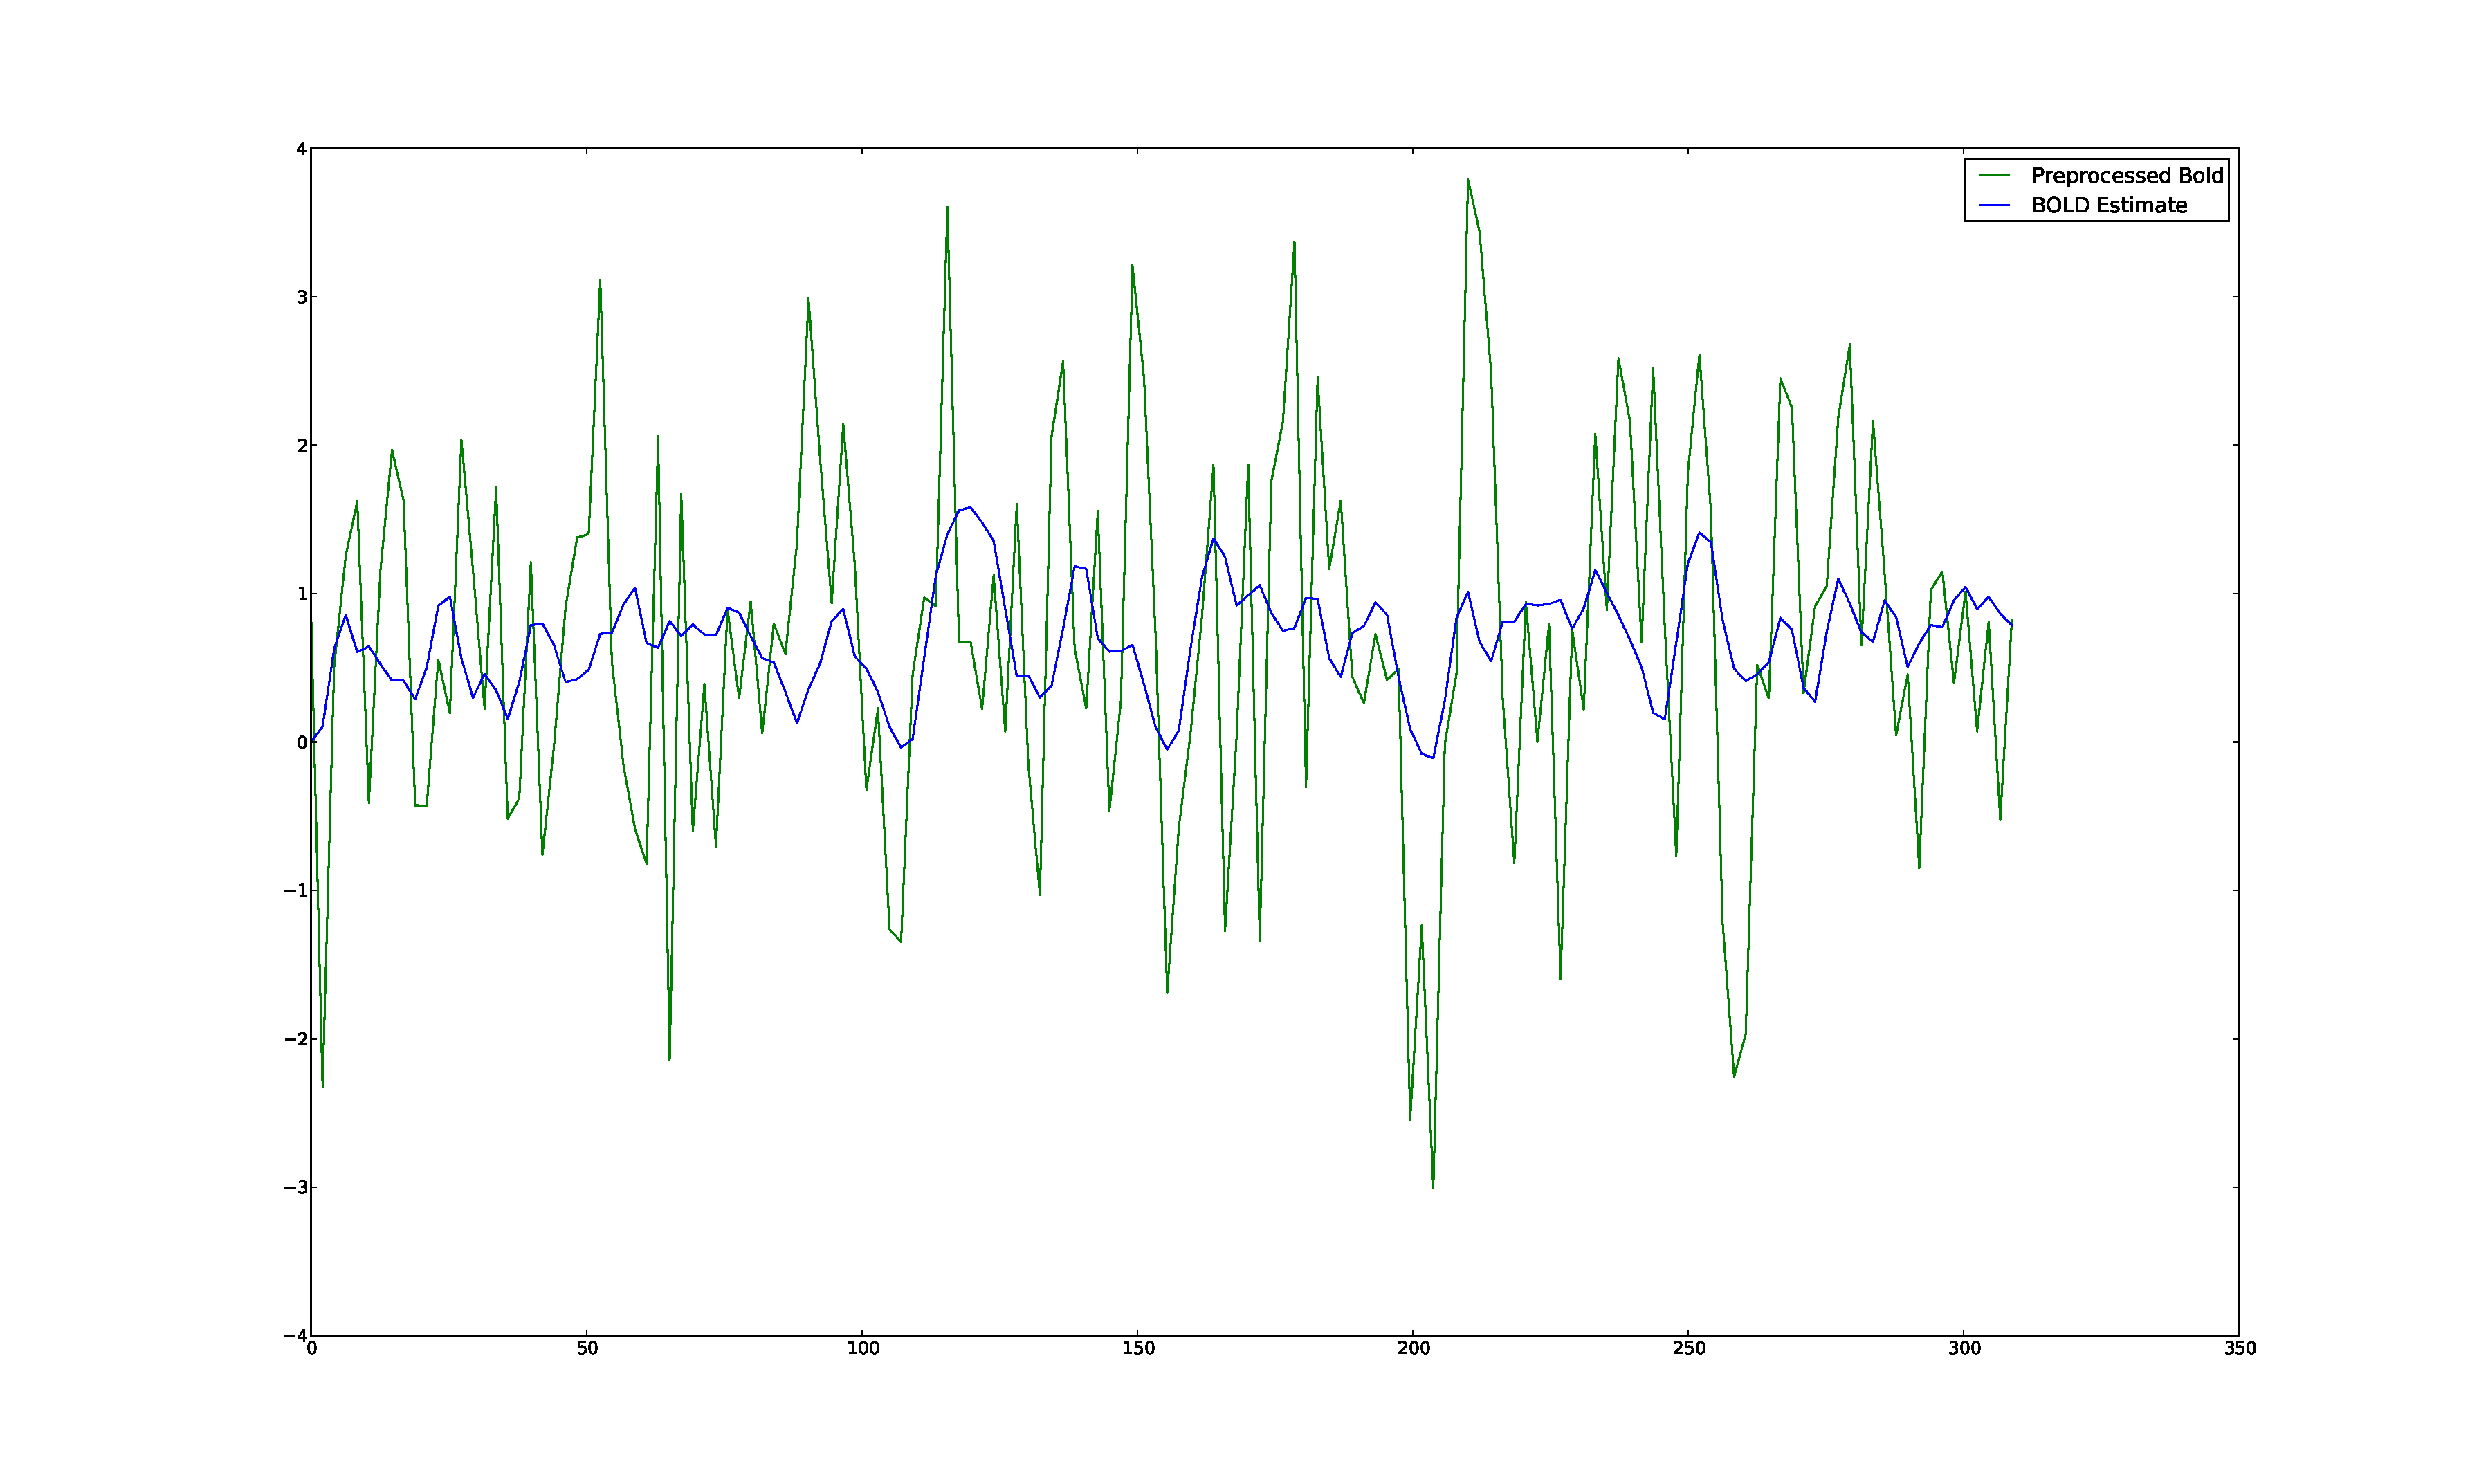
\includegraphics[clip=true,trim=5cm 2.5cm 4cm 3cm,width=.93\textwidth]{images/4_spm_26_15_7}}
\caption[Time Series Comparison, Section 4]{Time Series Comparison, Section 4.
Estimated vs. Actual \ac{BOLD} response. $t$-Score: $0.50$, \ac{MI}: $0.06$, Residual: $0.95$. }
\label{fig:comp4}
\end{figure}

% or in original coordinates 29-9-13
\begin{figure}
\centering
\subfigure[Particle Filter]{\label{fig:comp5pfilter} 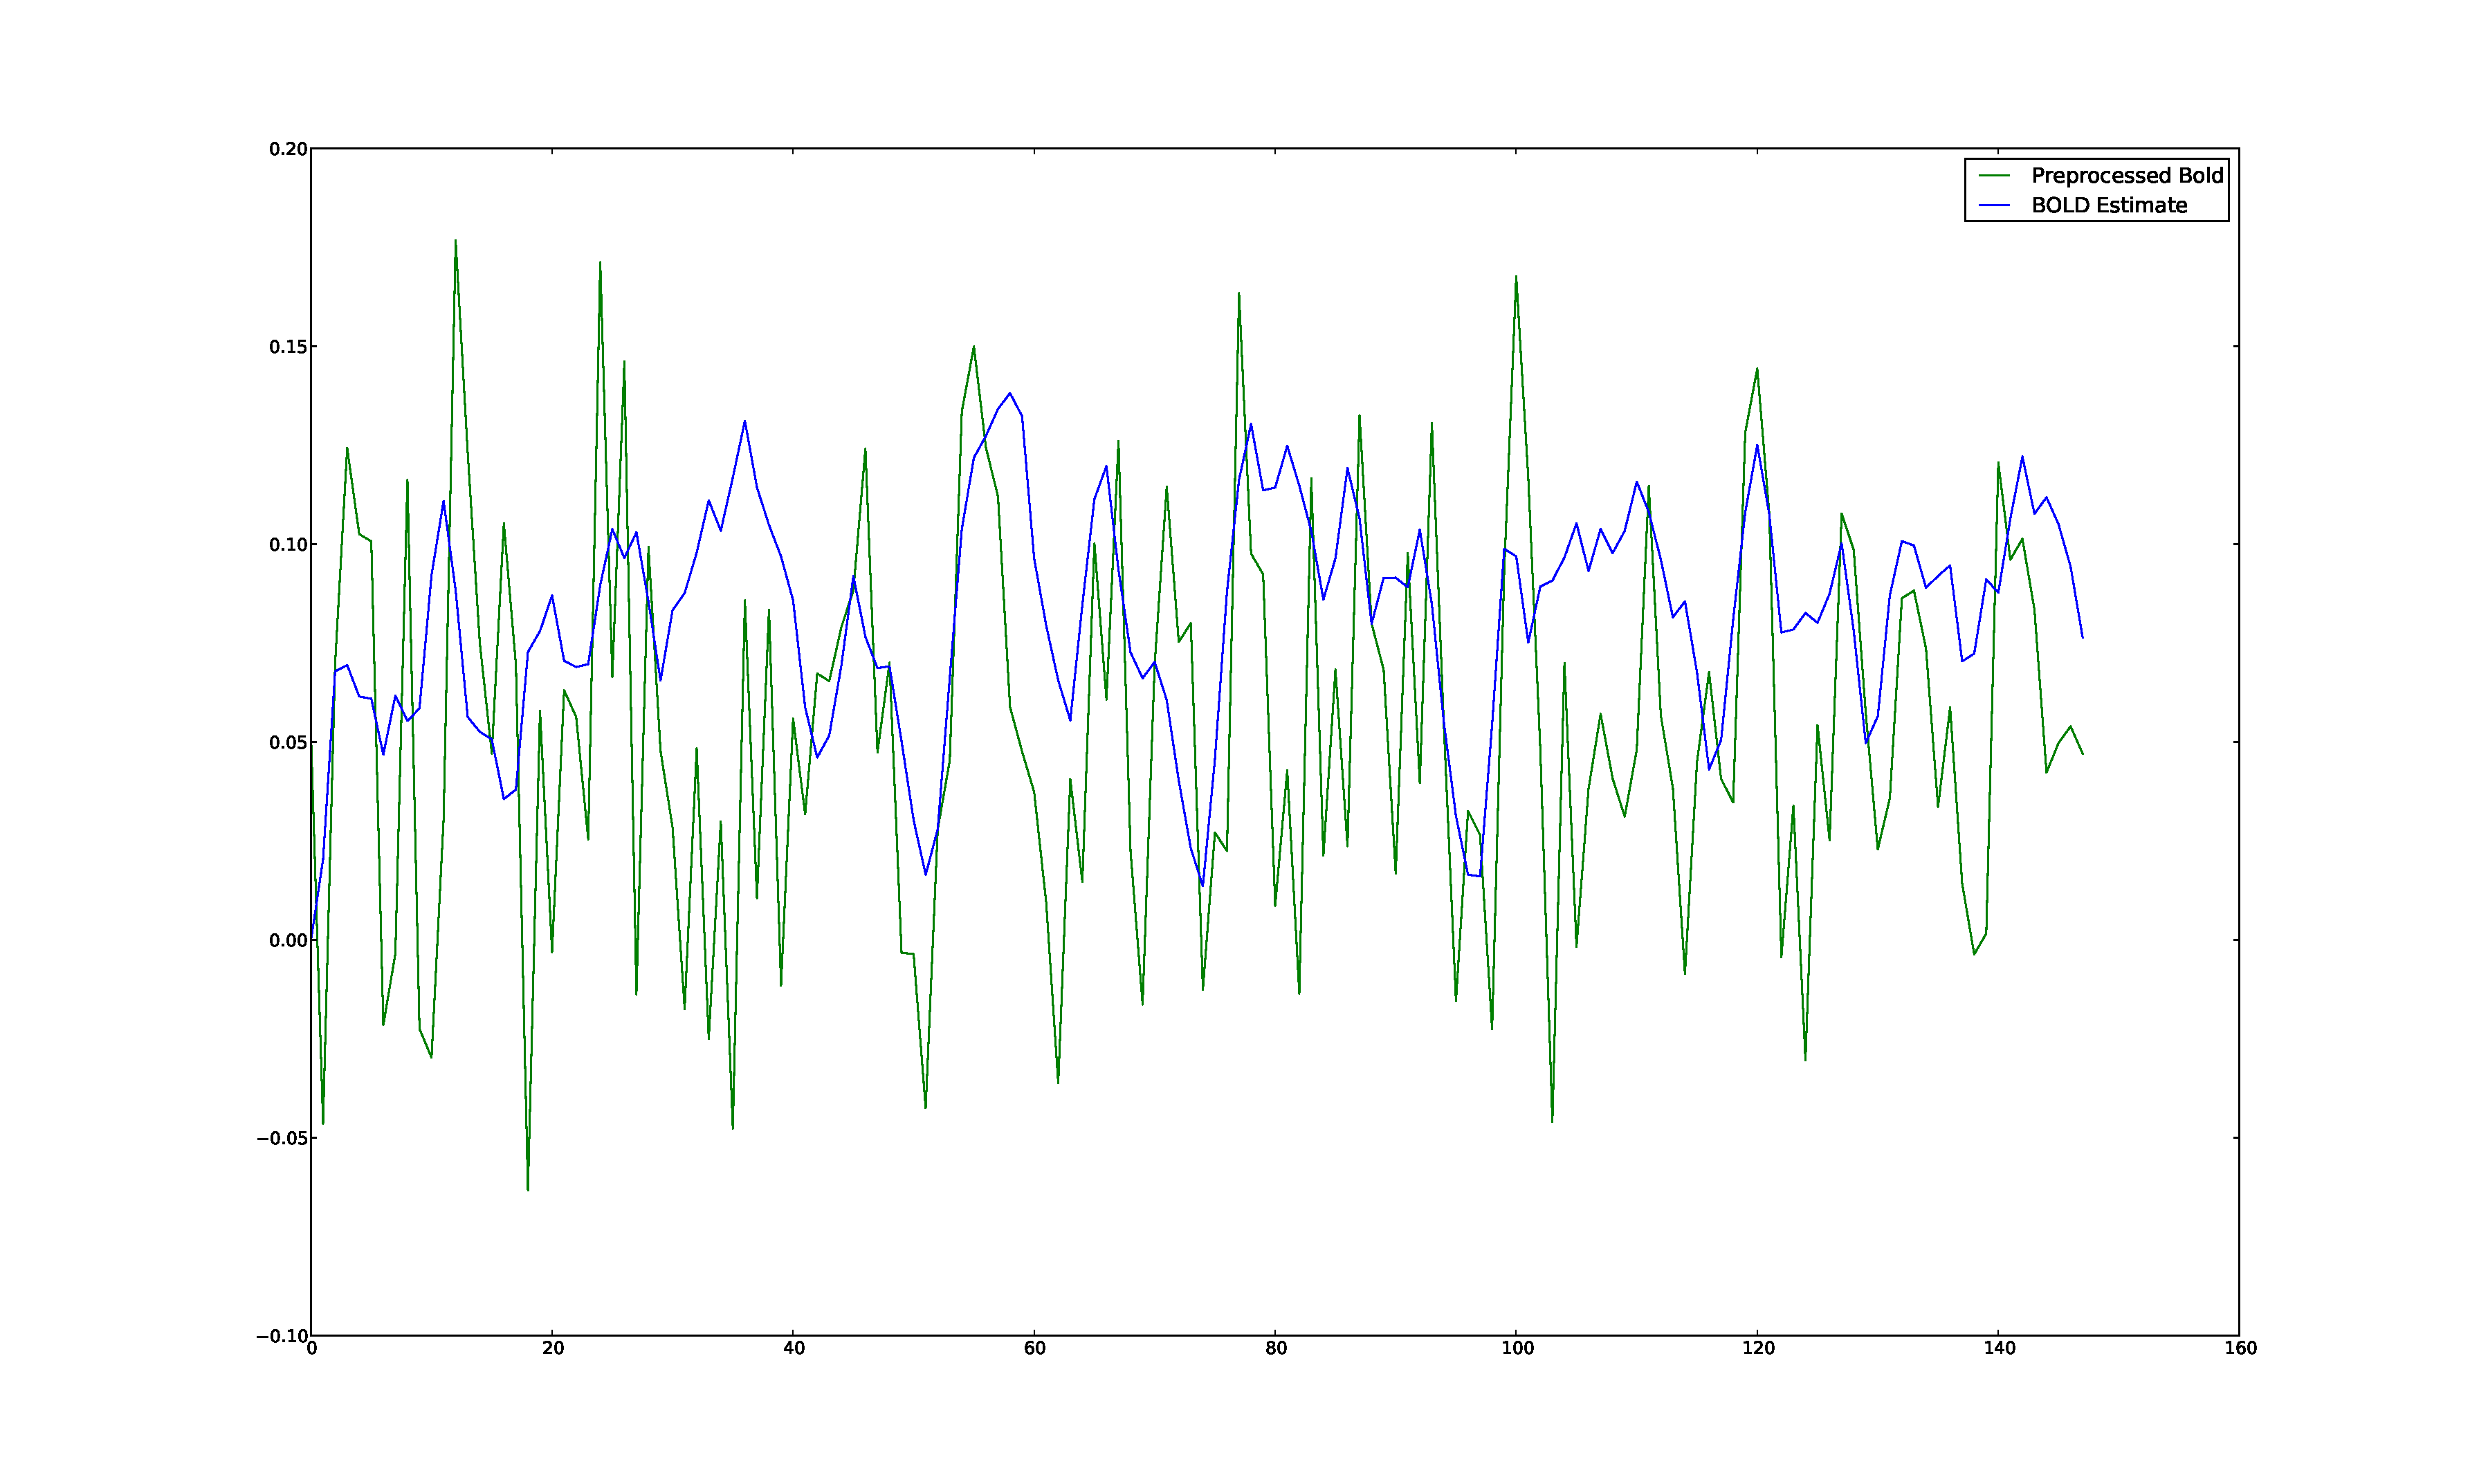
\includegraphics[clip=true,trim=5cm 2.5cm 4cm 3cm,width=.93\textwidth]{images/5_pfilter_29_9_13}}\\
\subfigure[SPM]{\label{fig:comp5spm} 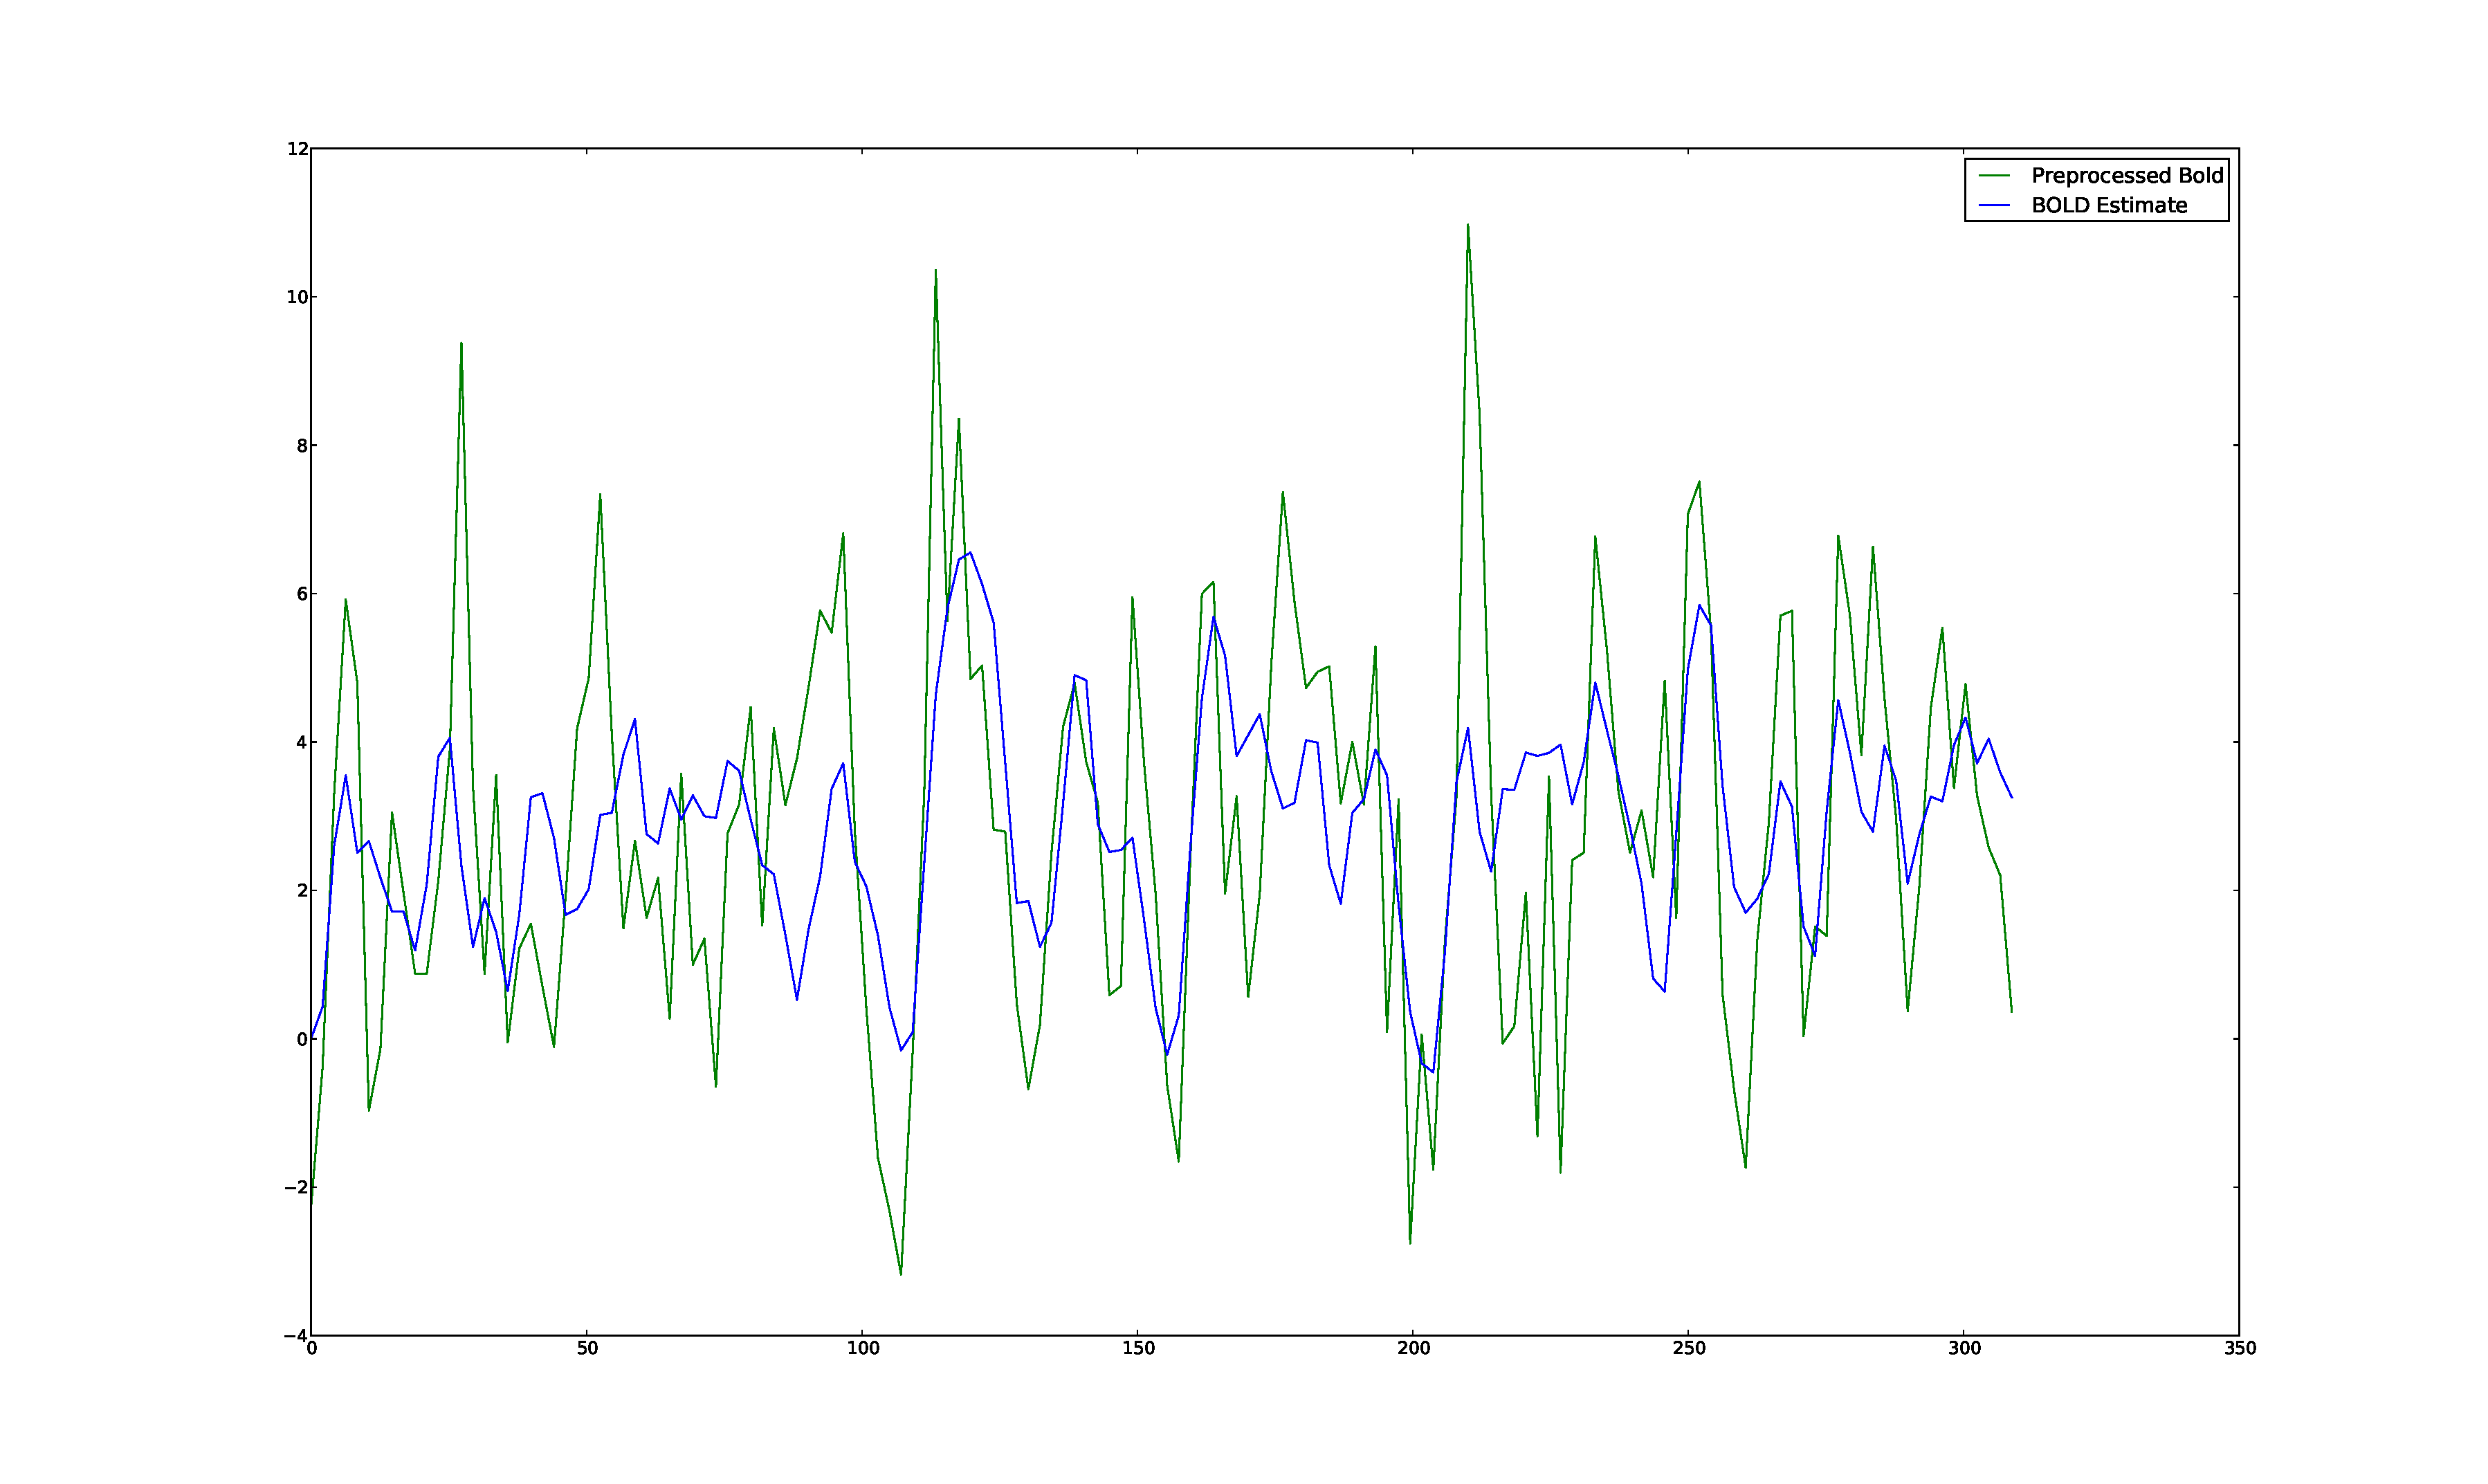
\includegraphics[clip=true,trim=5cm 2.5cm 4cm 3cm,width=.93\textwidth]{images/5_spm_29_9_13}}
\caption[Time Series Comparison, Section 5]{Time Series Comparison, Section 5.
Estimated vs. Actual \ac{BOLD} Response. $t$-Score: $4.17$, \ac{MI}: $0.02$, Residual: $1.14$.}
%\caption{Section 5, Below threshold in both particle filter checks, but above threshold in SPM. \ac{MI} of $0.0212822$, $t$-Value
%of $4.17399$ and $MSE$ of $1.14171$.}
\label{fig:comp5}
\end{figure}

%23-10-18 or in original coordinates 36-17-19
\begin{figure}
\centering
\subfigure[Particle Filter]{\label{fig:comp6pfilter} 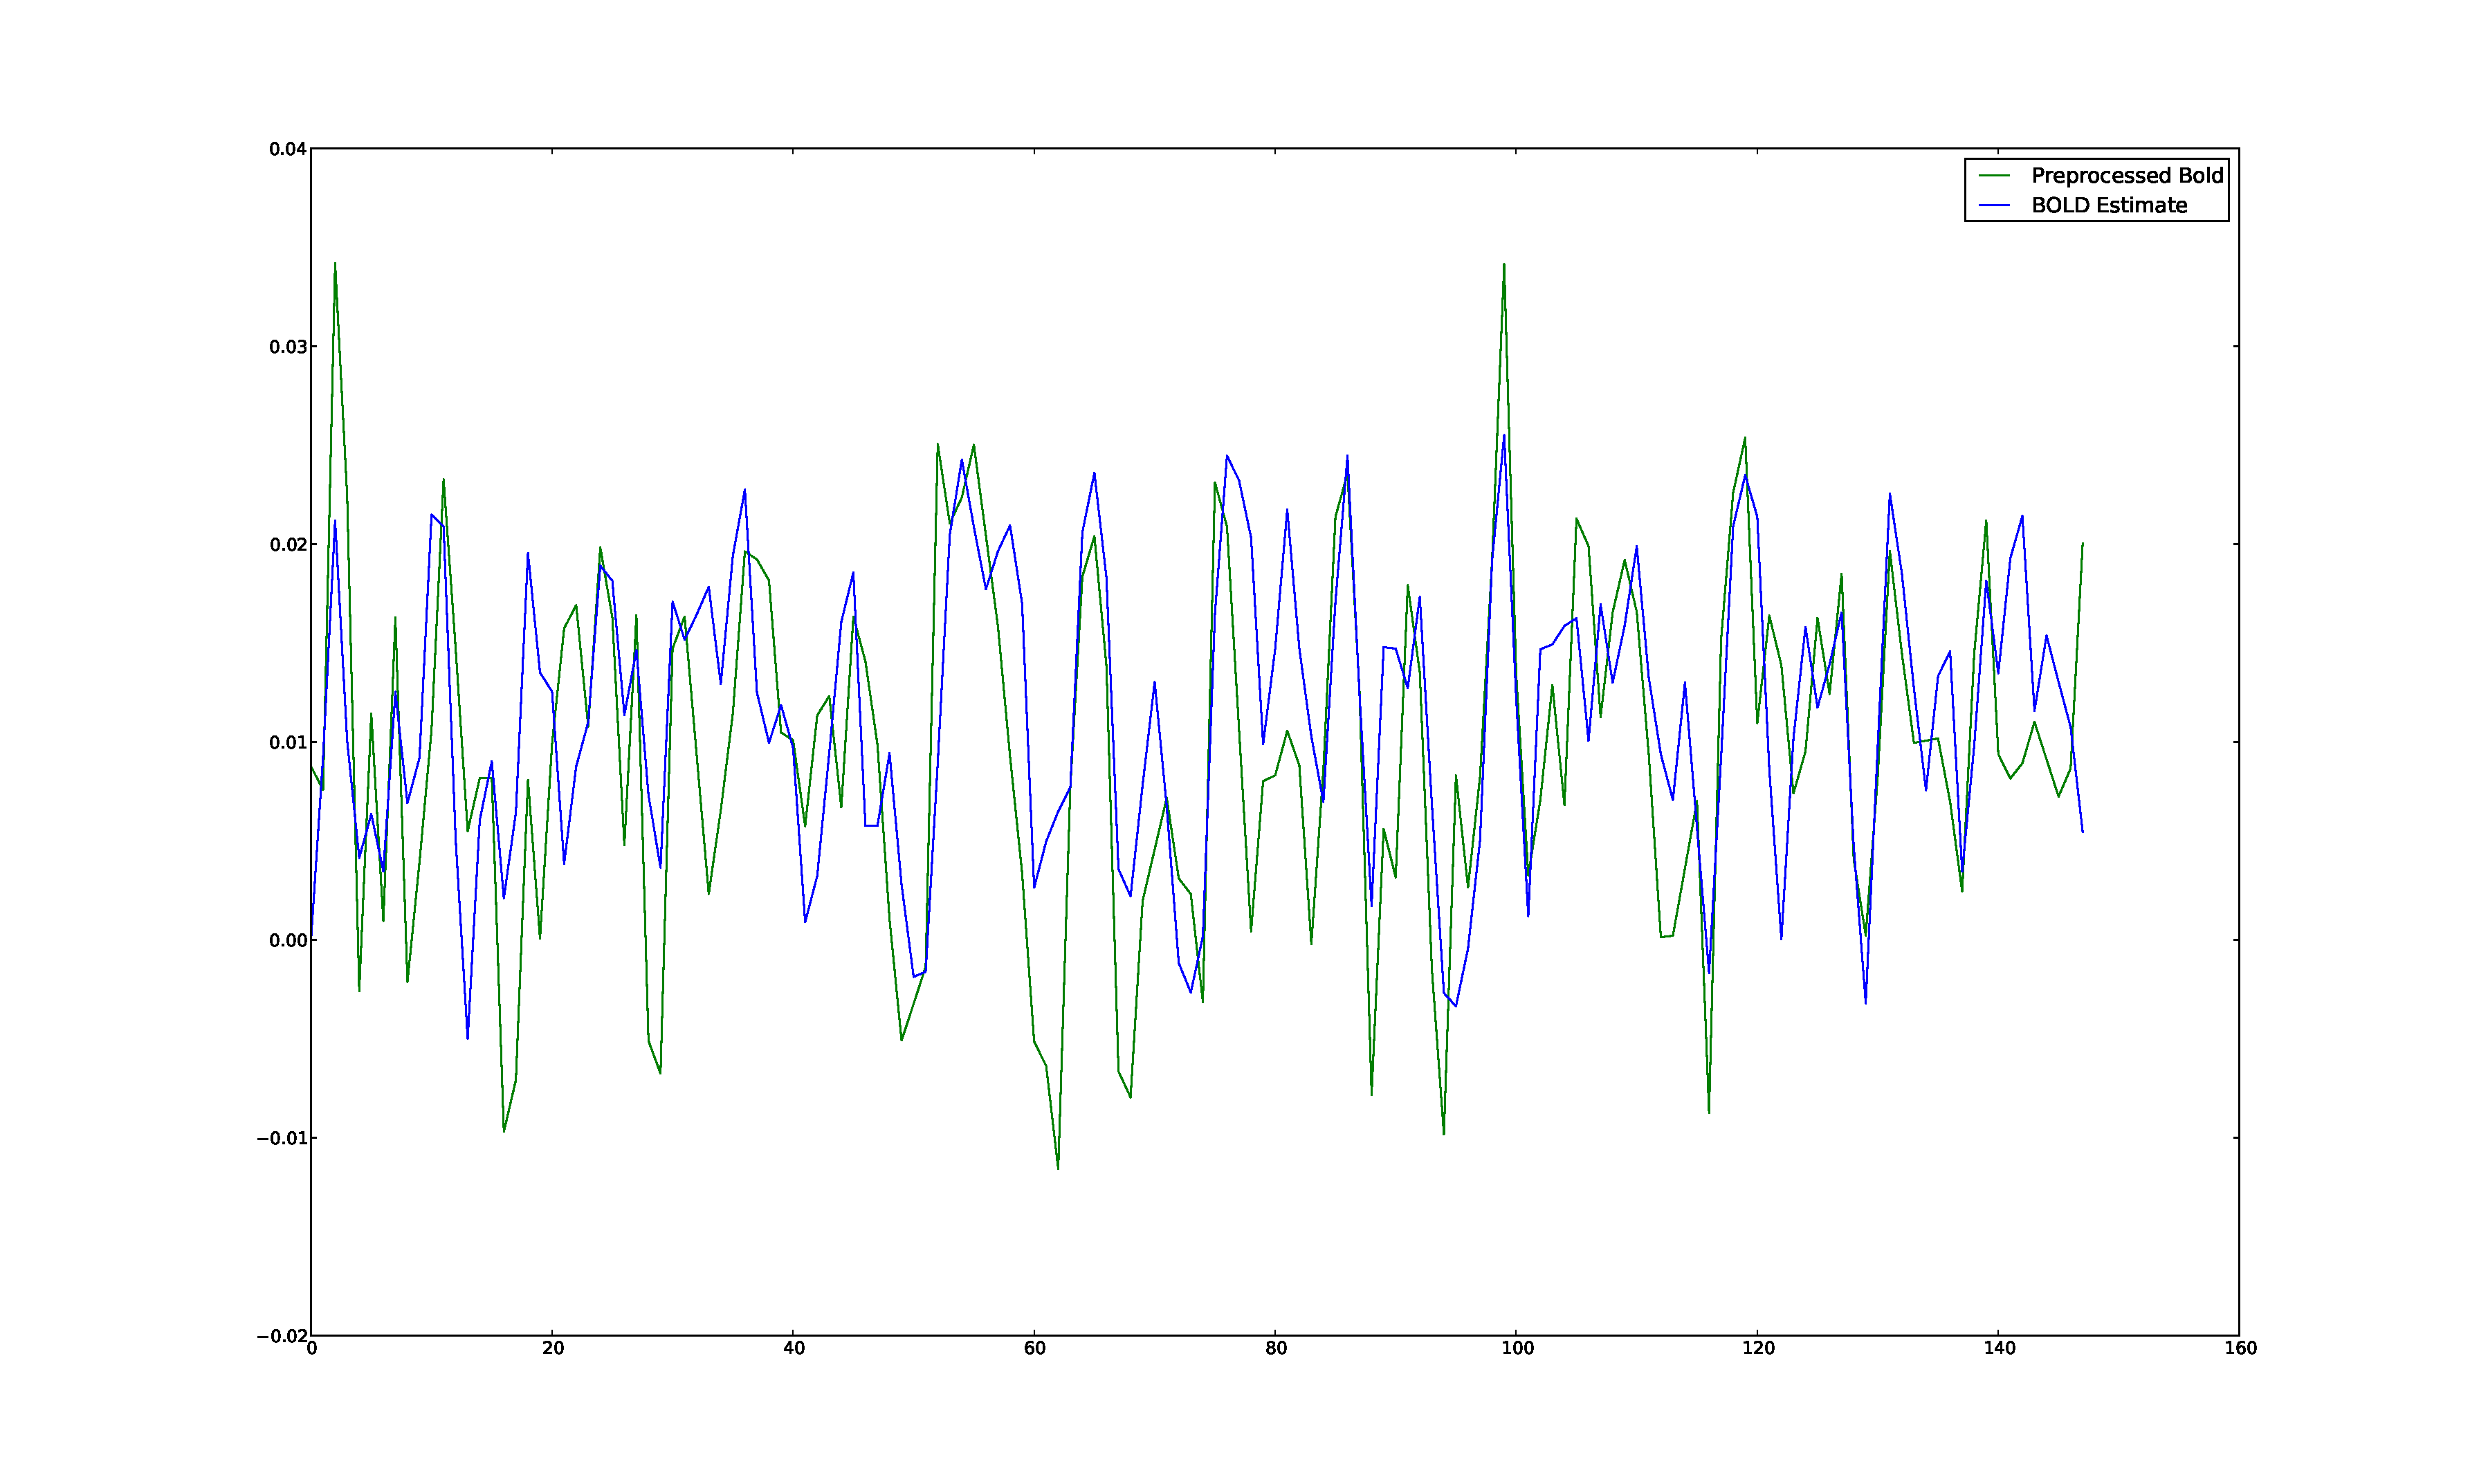
\includegraphics[clip=true,trim=5cm 2.5cm 4cm 3cm,width=.93\textwidth]{images/6_pfilter_36_17_19}}
\subfigure[SPM]{\label{fig:comp6spm} 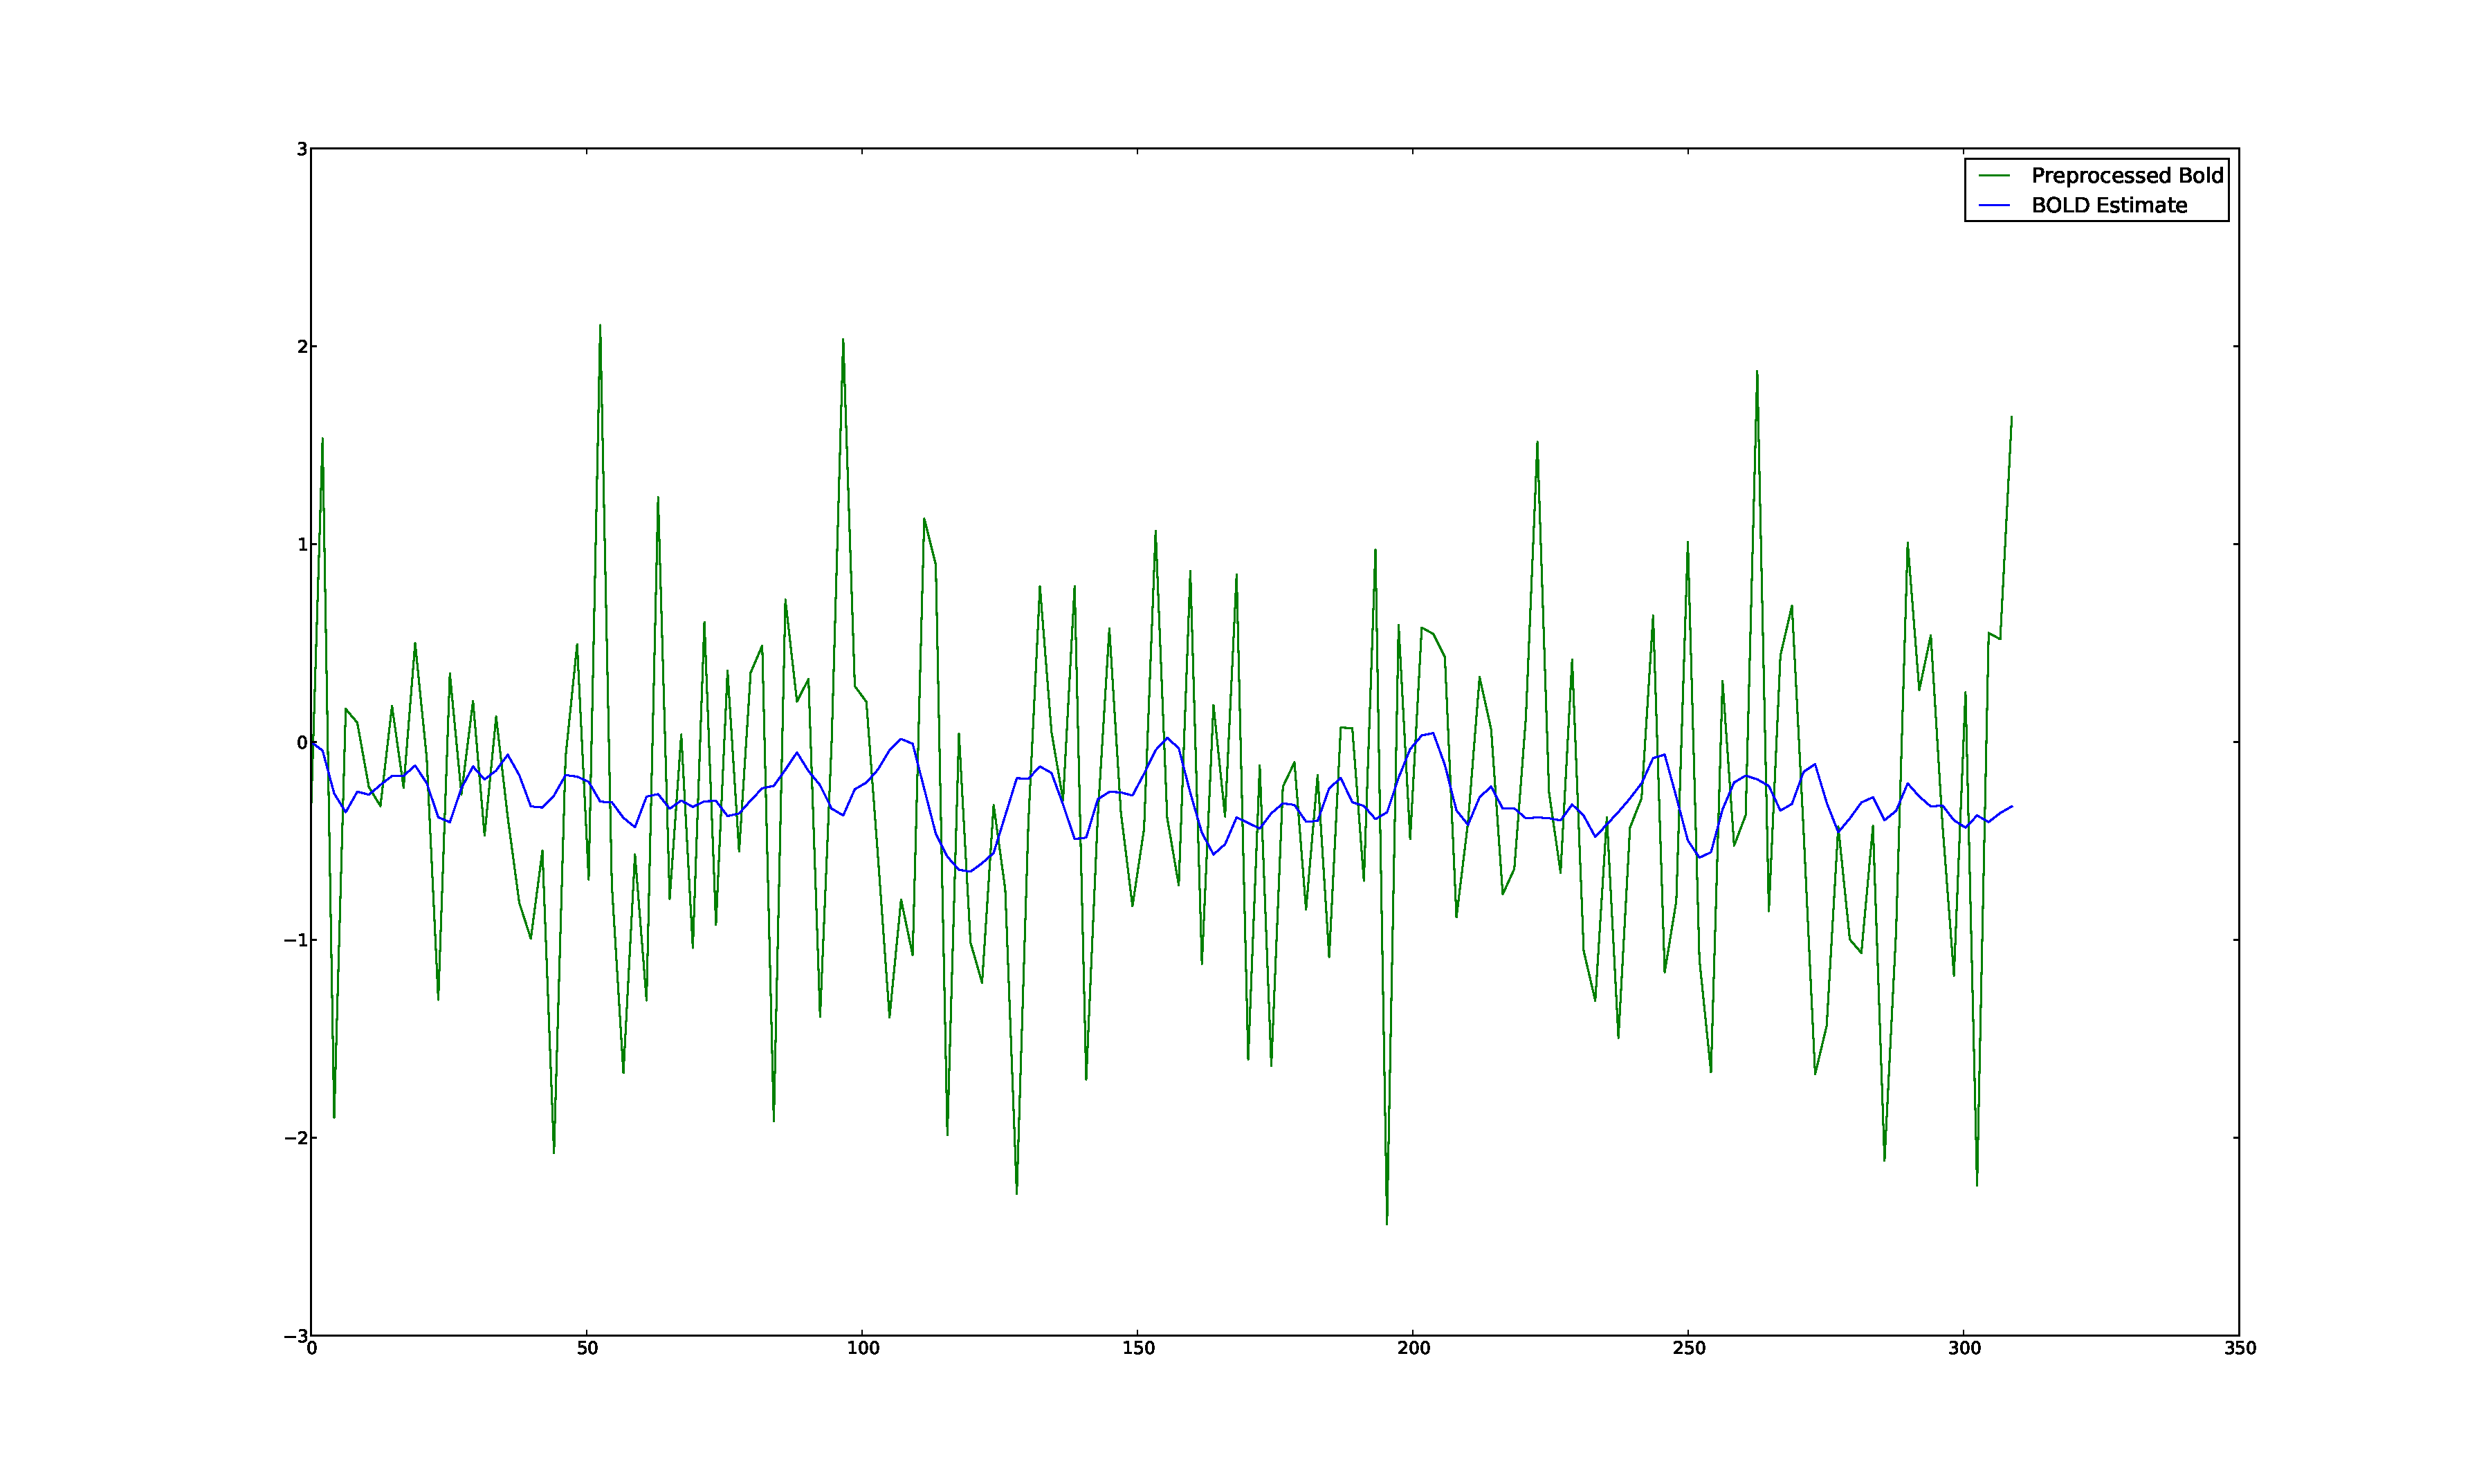
\includegraphics[clip=true,trim=5cm 2.5cm 4cm 3cm,width=.93\textwidth]{images/6_spm_36_17_19}}
\caption[Time Series Comparison, Section 6]{Time Series Comparison, Section 6.
Estimated vs. Actual \ac{BOLD} Response. $t$-Score: $2.49$, \ac{MI}: $.34$, Residual: $0.78$.}
%\caption{Section 6, MI of $0.335504$, T Value: $2.49154$, normalized error: $0.783348$ Not visible in SPM}
\label{fig:comp6}
\end{figure}

%16-19-0 or in original coordinates 29-26-1
\begin{figure}
\centering
\subfigure[Particle Filter]{\label{fig:comp7pfilter} 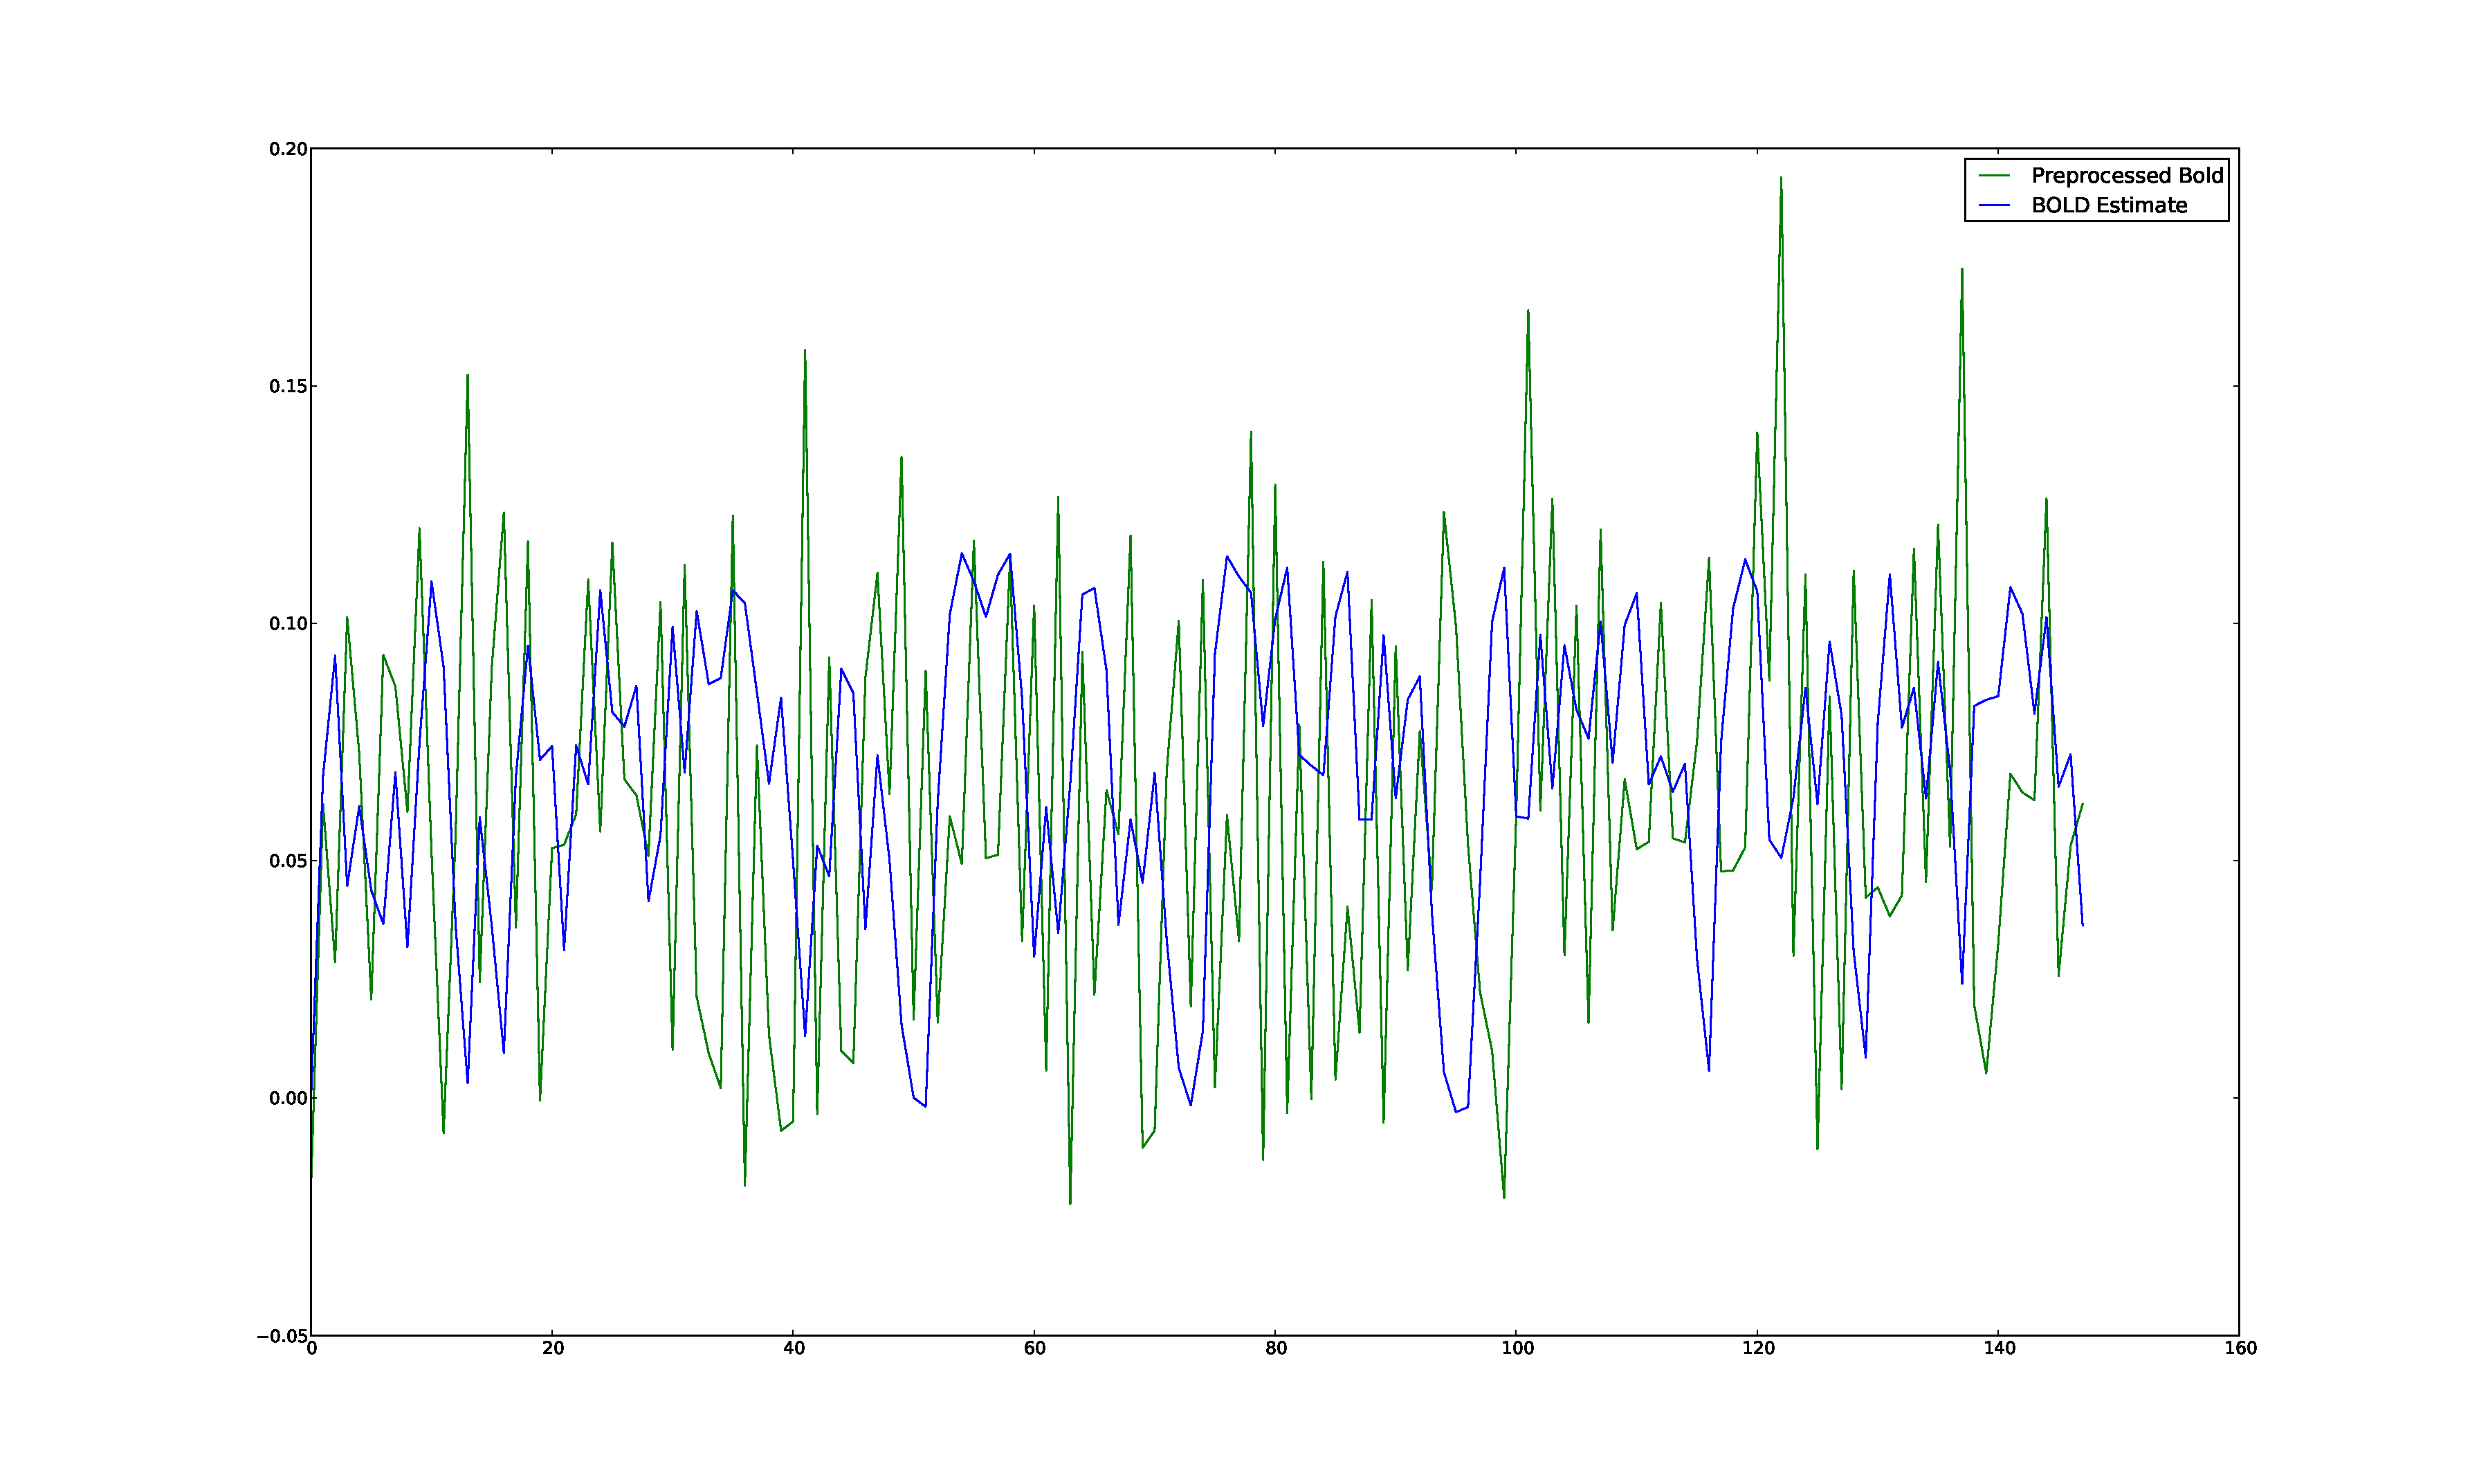
\includegraphics[clip=true,trim=5cm 2.5cm 4cm 3cm,width=.93\textwidth]{images/7_pfilter_29_26_1}}
%\subfigure[SPM]{\label{fig:comp7spm} 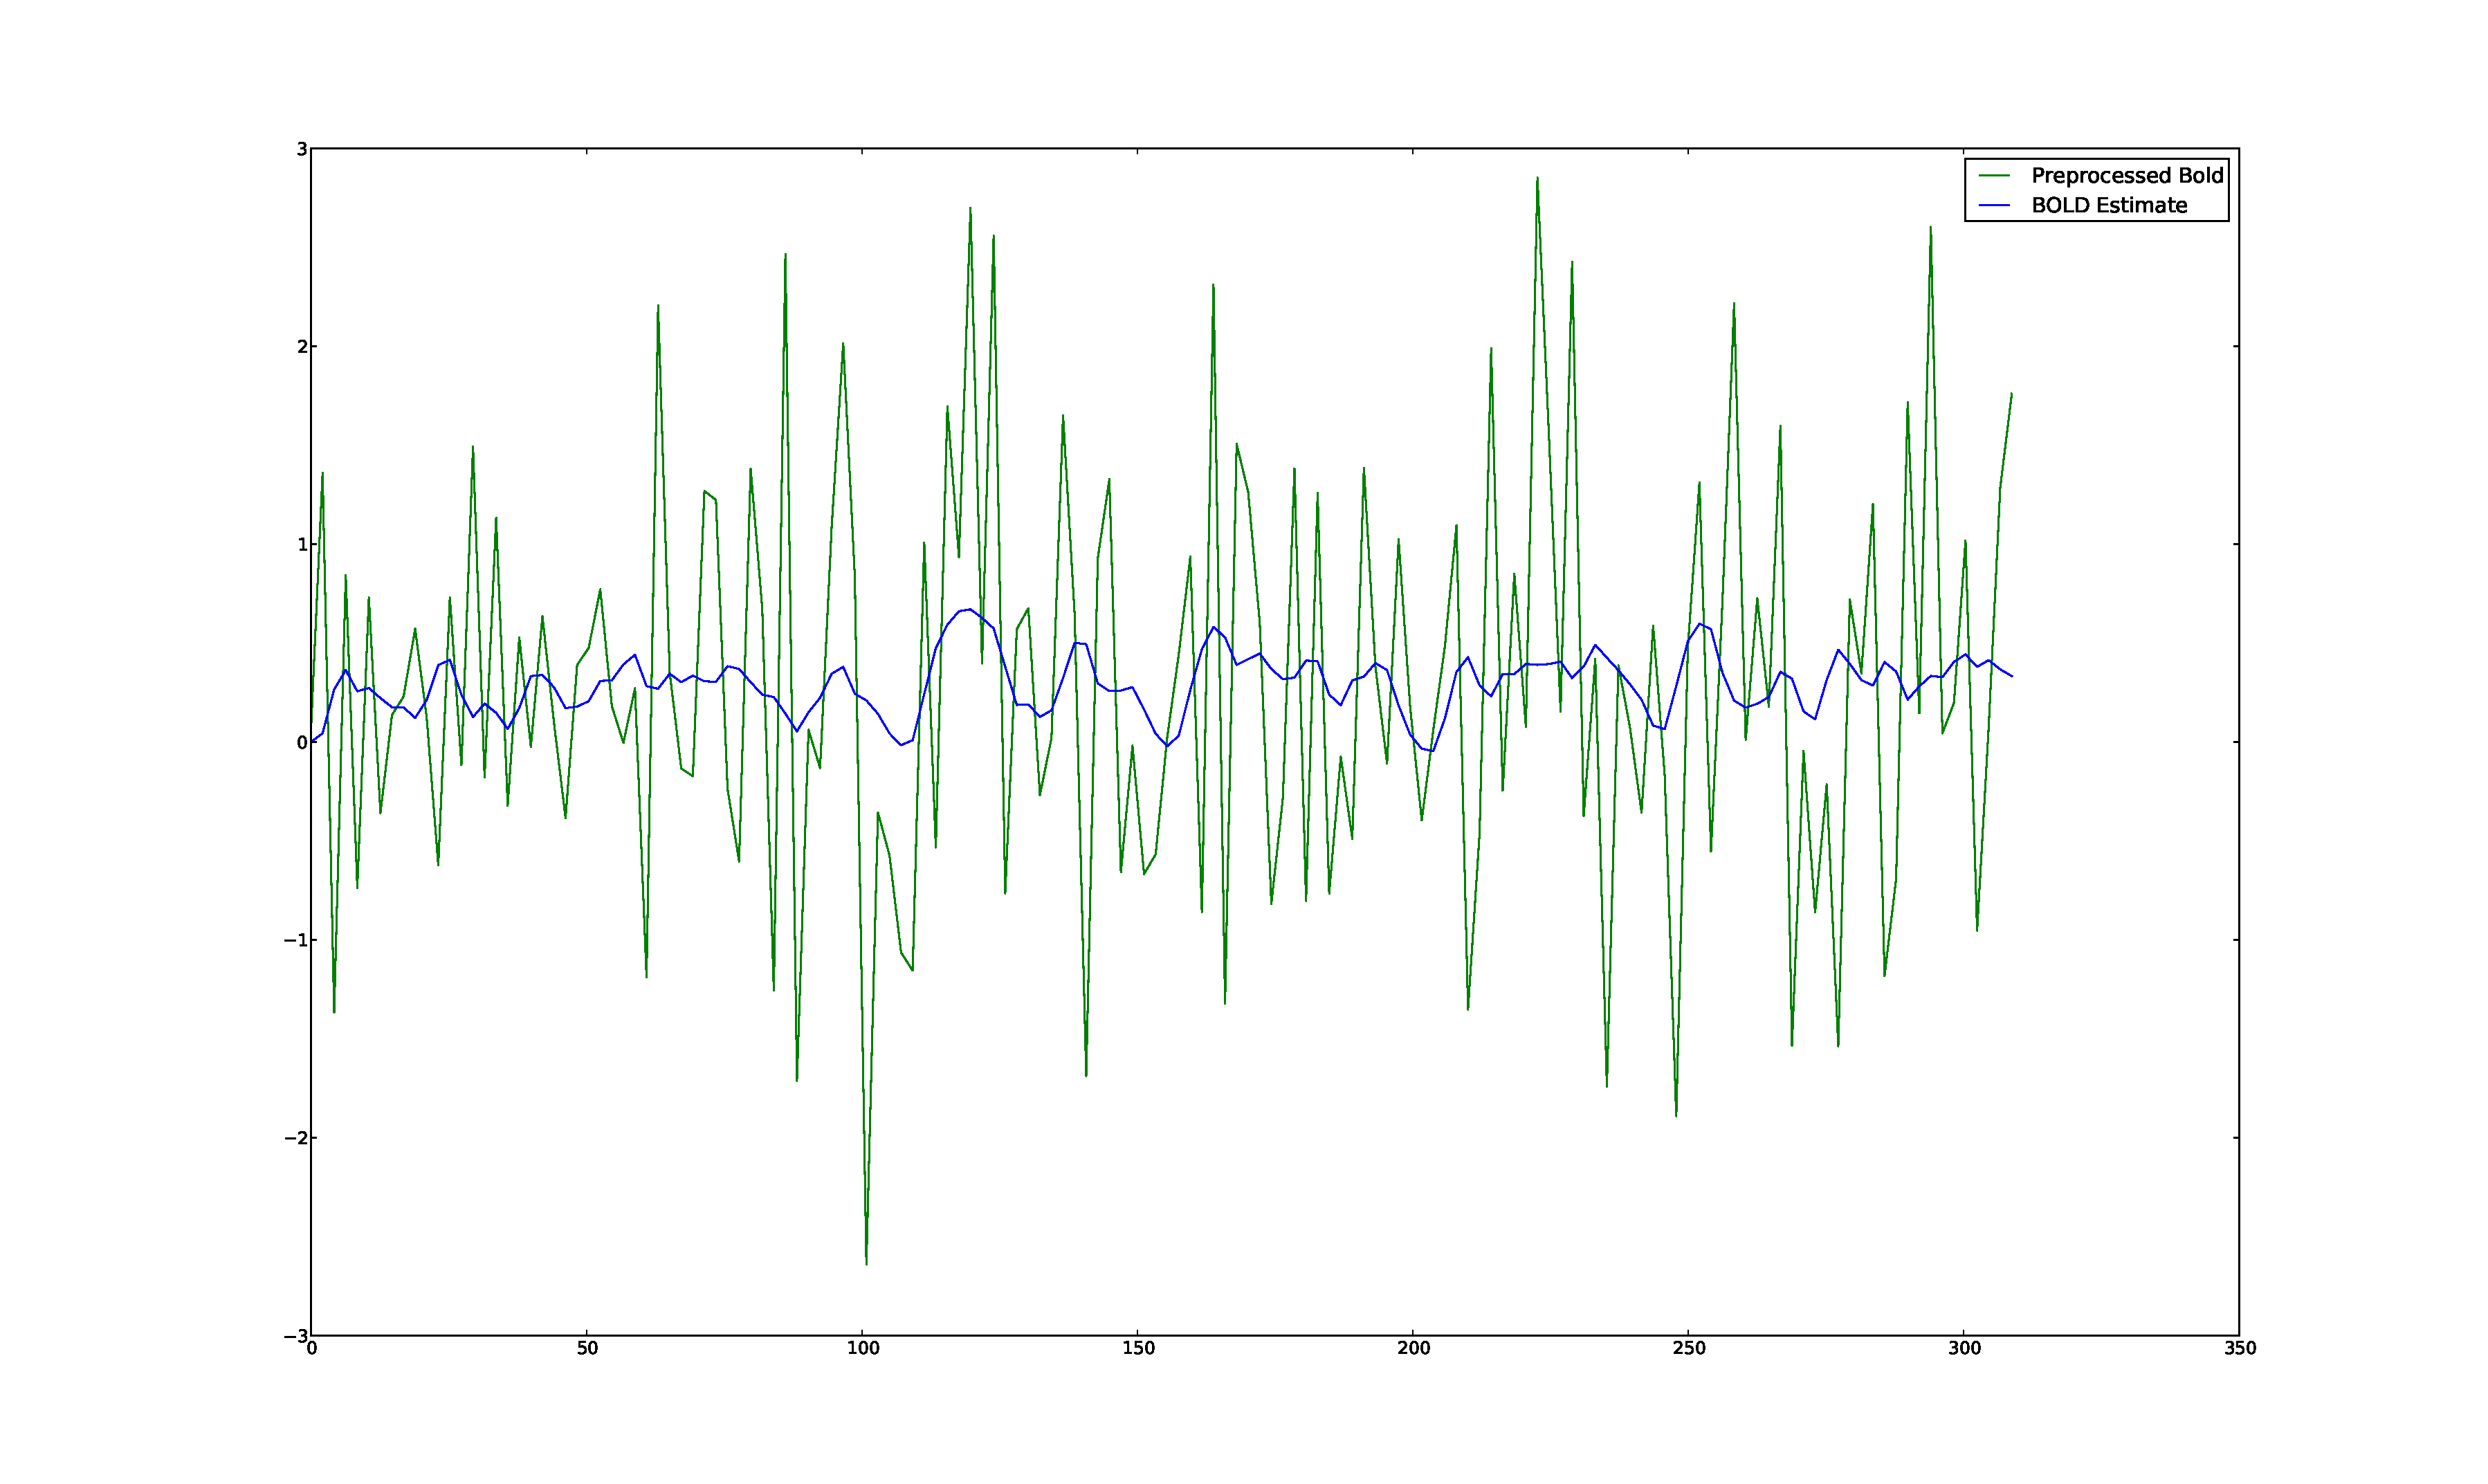
\includegraphics[clip=true,trim=5cm 2.5cm 4cm 3cm,width=.93\textwidth]{images/5_spm_25_34_25}}
\caption[Time Series Comparison, Section 7]{Time Series Comparison, Section 7.
Estimated vs. Actual \ac{BOLD} Response. $t$-Score: $1.32$, \ac{MI}: $0.11$, Residual: $1.10$.}
%\caption{Section 7, $.1052$ in MI, $1.31534$ in SPM (which left this flat) and $1.09992$ normalized $\sqrt{MSE}$. Only visible in MI map. }
\label{fig:comp7}
\end{figure}

Several voxels were chosen for further investigation from \autoref{fig:hm_canon_pfilter} and \autoref{fig:hm_canon_spm}.

Section 1 (\autoref{fig:comp1}) had a very high $t$-score, high \ac{MI} and
a low error. Visual inspection makes it obvious that this voxel fits the \ac{BOLD} model. A region
such as this would be called strong activation by neurologists. The
reason for the cleaner looking signal in \ac{SPM} is the additional Gaussian spatial smoothing
applied in preprocessing. This
has allowed for an extremely good fit in \ac{SPM}, although the particle filter handles the noise
well.

Section 2 is a difficult voxel to assess (\autoref{fig:comp2}).
While certain peaks seem to correlate, overall
the particle filter input signal is extremely noisy.
This would appear to be a false positive on \ac{SPM}'s part because of the Gaussian smoothing.
This voxel is not being driven directly by the input, although it
could be gated or driven through intermediate region.

Section 3 and 4 are both examples of nearly pure-noise signals, at least from the standpoint
of the given stimulus (\autoref{fig:comp3}, \autoref{fig:comp4}).
These two voxels are false positives by the normalized residual.
Note that in both cases the \ac{MI} was extremely low, meaning that
according to the \ac{MI} these were not good fits. Both section 3 and 4 have
significant peaks, raising the question of whether they may be active,
but not correlated directly with the input.

It is questionable whether the fifth voxel should be considered inside the
brain; however, like section 2, \ac{SPM} deemed it active (\autoref{fig:comp5}).
Also like section 2, the most likely cause of the problem is the smoothing
applied for \ac{SPM}. There are certain peaks that certainly match the
\ac{BOLD} signal, yet that is only a small part of the whole.
Take for instance the measurements between $30$ and $40$ seconds.
In that interval there is a significant spike in the \ac{BOLD} signal, yet the
actual measured signal declines. This is an indication that the \ac{BOLD} signal is not directly
being driven by the input. The \ac{SPM} fit is not particularly good either,
with the $t$-score barely above the threshold of $4$.

Section 6 (\autoref{fig:comp6}) is a clear example of a false negative
from \ac{SPM}. The \ac{BOLD} model fit is extremely good, yet the \ac{SPM} signal looks completely
like noise. One possible reason for this is that the low peak signal ($<0.03$),
made it more susceptible to being smoothed out.

Section 7 is an ambiguous time series. While the thresholds applied here
are empirical, this voxel is on the borderline for both \ac{MI}
and the normalized residual.
This case is reminiscent of the pure-noise tests performed in the previous chapter,
and is a perfect example of the false positive problem.
The signal oscillates far faster than the \ac{BOLD} estimate, yet
somehow the \ac{MI} reaches $.1052$ and the normalized residual is just below $1.1$.

\section{Parameter Estimates}
\label{sec:Real Data Parameter Estimates}
Although the parameters are not uniquely identifiable by a single time-series, that
does not mean the estimates are useless . The parameters still contain useful
information about the system. Additionally, as an aggregate they form a distribution of
the feasible parameters parameters for a particular patient. Therefore
\autoref{fig:pmap0} through \autoref{fig:pmap6}
contain the parameter maps for the system and \autoref{fig:realhist} is a histogram across all voxels
for which the \ac{MI} was greater than $0.15$. As before, the threshold is not
scientifically derived, yet in tests this threshold provided a decent balance to remove most
of the questionably active voxels in the system.

\begin{figure}[H]
\centering
\subfigure{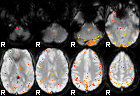
\includegraphics[width=13cm]{images/pmap0}}
\subfigure{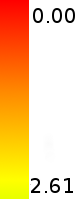
\includegraphics[scale=.5]{images/pscale_00}}
\caption{Regional $\tau_0$ Estimates}
\label{fig:pmap0}
\end{figure}

\begin{figure}[H]
\centering
\subfigure{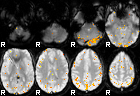
\includegraphics[width=13cm]{images/pmap1}}
\subfigure{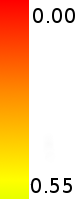
\includegraphics[scale=.5]{images/pscale_01}}
\caption{Regional $\alpha$ Estimates}
\label{fig:pmap1}
\end{figure}

\begin{figure}[H]
\centering
\subfigure{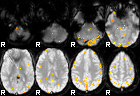
\includegraphics[width=13cm]{images/pmap2}}
\subfigure{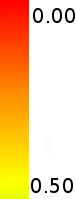
\includegraphics[scale=.5]{images/pscale_02}}
\caption{Regional $E_0$ Estimates}
\label{fig:pmap2}
\end{figure}

\begin{figure}[H]
\centering
\subfigure{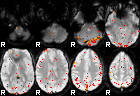
\includegraphics[width=13cm]{images/pmap3}}
\subfigure{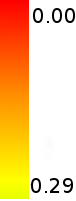
\includegraphics[scale=.5]{images/pscale_03}}
\caption{Regional $V_0$ Estimates}
\label{fig:pmap3}
\end{figure}

\begin{figure}[H]
\centering
\subfigure{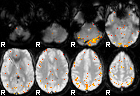
\includegraphics[width=13cm]{images/pmap4}}
\subfigure{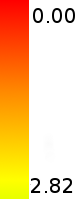
\includegraphics[scale=.5]{images/pscale_04}}
\caption{Regional $\tau_f$ Estimates}
\label{fig:pmap4}
\end{figure}

\begin{figure}[H]
\centering
\subfigure{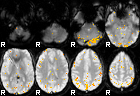
\includegraphics[width=13cm]{images/pmap5}}
\subfigure{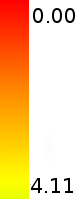
\includegraphics[scale=.5]{images/pscale_05}}
\caption{Regional $\tau_s$ Estimates}
\label{fig:pmap5}
\end{figure}

\begin{figure}[H]
\centering
\subfigure{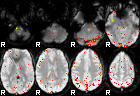
\includegraphics[width=13cm]{images/pmap6}}
\subfigure{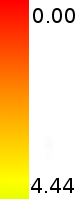
\includegraphics[scale=.5]{images/pscale_06}}
\caption{Regional $\epsilon$ Estimates}
\label{fig:pmap6}
\end{figure}

Regions with poor fit cannot have reliable parameter estimates because the input did not meaningfully
correlate input with output, which is why a threshold was applied.
\ac{MI} was chosen over the residual because the
maps had more coherency, and had less error in slice simulations (\autoref{fig:sim_hm2} vs.
\autoref{fig:simslice_hm_res}).

\begin{figure}
\centering
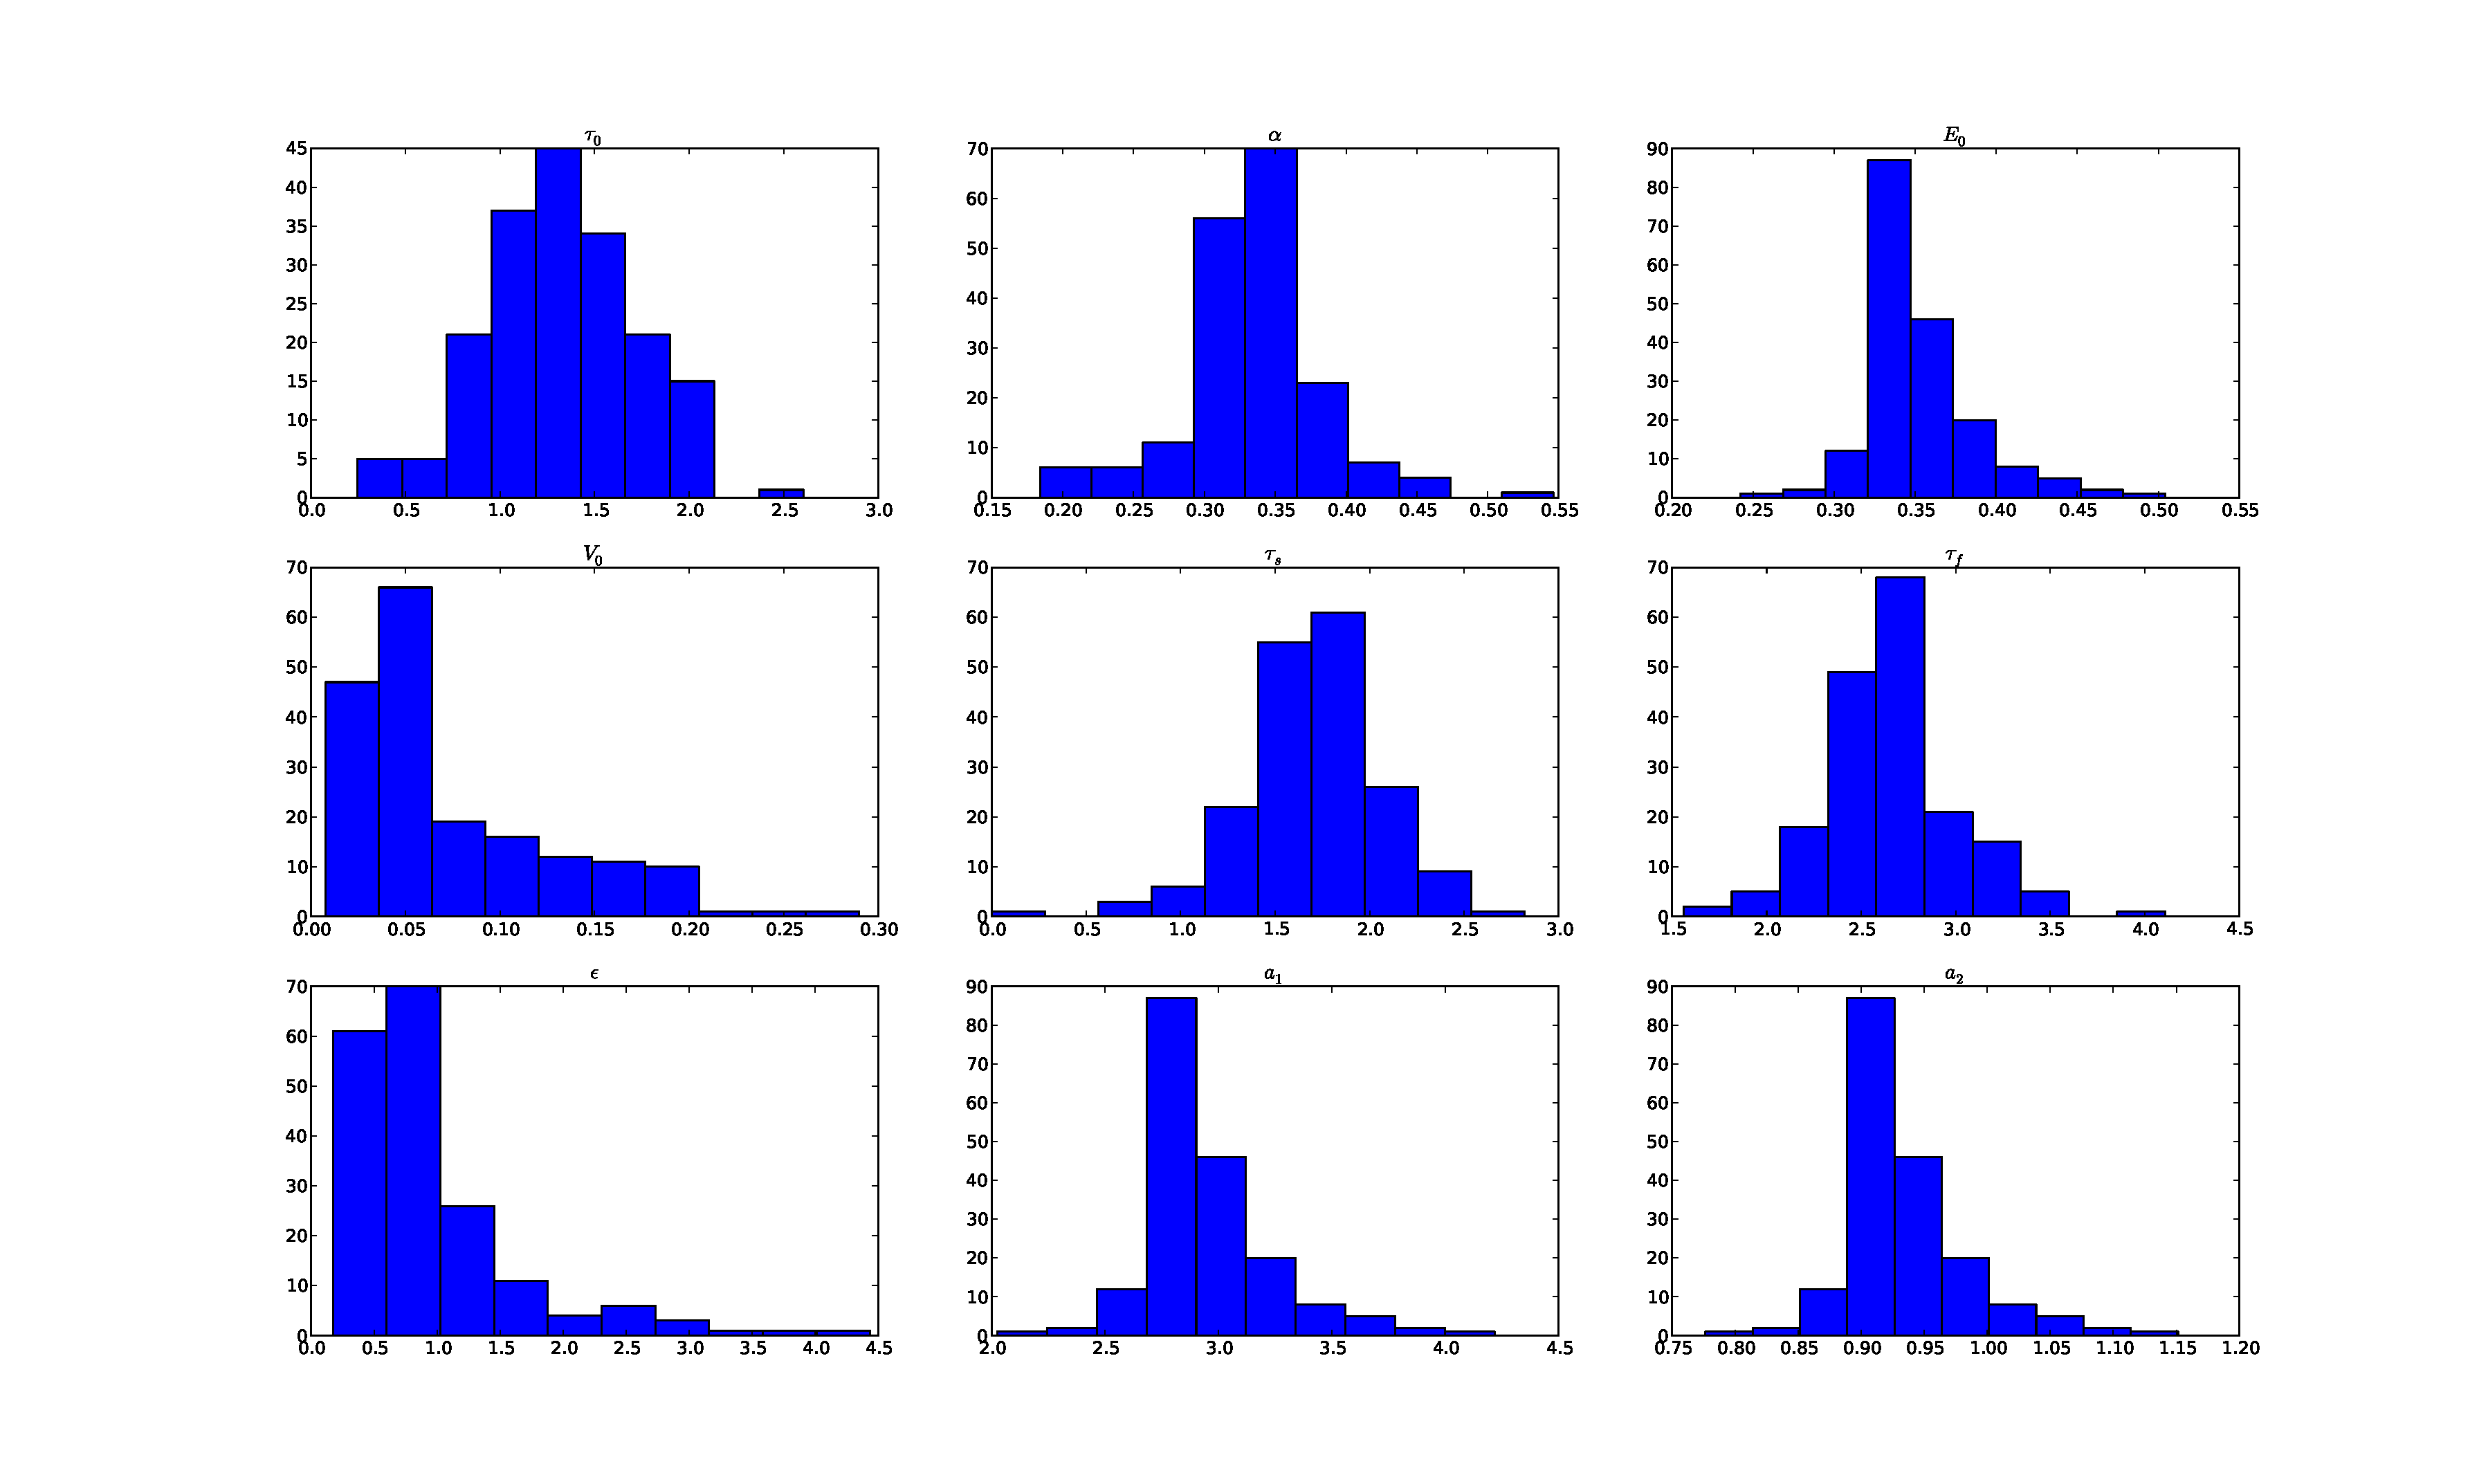
\includegraphics[clip=true,trim=6cm 1cm 5cm 1cm,width=\textwidth]{images/realhist}
\caption{Histogram of parameters in active regions (\acs{MI} $> .15$) overlayed
with the parameter estimates from Friston et al. \cite{Friston2002b}}
\label{fig:realhist}
\end{figure}

The histograms show variance higher than the prior, indicating that
parameters are migrating quite a bit during particle filter convergence.
It can be said that all of these regions had relatively accurate \ac{BOLD}
measurements, and yet the final parameter estimates vary widely.

\section{Discussion}
The activation maps generated by the particle filter are very similar
to those produced by \ac{SPM}. This indicates that the particle filter is
successfully estimating the \ac{BOLD} output, in spite of the lack of spatial
smoothing. Comparing the \acl{MI} metric with the normalized residual,
\ac{MI} gives much better clusters, although that doesn't necessarily mean it
is better. Although many of the differences between \ac{SPM} and the particle filter
were driven by differences in preprocessing, it is worth noting that
the preprocessing applied by \ac{SPM} is necessary for \ac{SPM} to give decent results.
Without spatial smoothing \ac{SPM} is unable to cope with additional noise, and
gives significant numbers of false positives.
Although the parameter maps have some spatial coherence, the histograms
of the parameters still indicate that the parameters are under-determined.
